% Seminar 4: Cozi Grele --- Skew-t, GED și EVT

\documentclass[9pt, aspectratio=169, t]{beamer}
%=============================================================================
% PREAMBUL COMUN - Statistica Piețelor Financiare
% Prezentări academice de calitate Harvard
% Program de licență, Academia de Studii Economice din București
%
% Utilizare: \documentclass[9pt, aspectratio=169, t]{beamer}
%            %=============================================================================
% PREAMBUL COMUN - Statistica Piețelor Financiare
% Prezentări academice de calitate Harvard
% Program de licență, Academia de Studii Economice din București
%
% Utilizare: \documentclass[9pt, aspectratio=169, t]{beamer}
%            %=============================================================================
% PREAMBUL COMUN - Statistica Piețelor Financiare
% Prezentări academice de calitate Harvard
% Program de licență, Academia de Studii Economice din București
%
% Utilizare: \documentclass[9pt, aspectratio=169, t]{beamer}
%            \input{preamble}
%            \subtitle{Seminar X: Titlul Seminarului}
%            \begin{document} ...
%=============================================================================

% Asigură încadrarea conținutului pe diapozitive
\setbeamersize{text margin left=8mm, text margin right=8mm}

%=============================================================================
% CONFIGURARE TEMĂ ȘI STIL
%=============================================================================
\usetheme{default}

% Paletă de Culori
\definecolor{MainBlue}{RGB}{26, 58, 110}
\definecolor{AccentBlue}{RGB}{26, 58, 110}
\definecolor{IDAred}{RGB}{205, 0, 0}
\definecolor{DarkGray}{RGB}{51, 51, 51}
\definecolor{MediumGray}{RGB}{128, 128, 128}
\definecolor{LightGray}{RGB}{248, 248, 248}
\definecolor{VeryLightGray}{RGB}{235, 235, 235}
\definecolor{KeynoteGray}{RGB}{218, 218, 218}
\definecolor{SectionGray}{RGB}{120, 120, 120}
\definecolor{FooterGray}{RGB}{100, 100, 100}
\definecolor{Crimson}{RGB}{220, 53, 69}
\definecolor{Forest}{RGB}{46, 125, 50}
\definecolor{Amber}{RGB}{181, 133, 63}
\definecolor{Orange}{RGB}{230, 126, 34}
\definecolor{Purple}{RGB}{142, 68, 173}

% Fundal gradient (gradient Keynote exact 315°: alb la RGB 218,218,218)
\setbeamertemplate{background}{%
    \begin{tikzpicture}[remember picture, overlay]
        \shade[shading=axis, shading angle=315,
        top color=white, bottom color=KeynoteGray]
        (current page.south west) rectangle (current page.north east);
    \end{tikzpicture}%
}
% Culoare solidă de rezervă pentru compatibilitate
\setbeamercolor{background canvas}{bg=}

\setbeamercolor{palette primary}{bg=MainBlue, fg=white}
\setbeamercolor{palette secondary}{bg=MainBlue!85, fg=white}
\setbeamercolor{palette tertiary}{bg=MainBlue!70, fg=white}
\setbeamercolor{structure}{fg=MainBlue}
\setbeamercolor{title}{fg=IDAred}
\setbeamercolor{frametitle}{fg=IDAred, bg=}
\setbeamercolor{block title}{bg=MainBlue, fg=white}
\setbeamercolor{block body}{bg=VeryLightGray, fg=DarkGray}
\setbeamercolor{block title alerted}{bg=Crimson, fg=white}
\setbeamercolor{block body alerted}{bg=Crimson!8, fg=DarkGray}
\setbeamercolor{block title example}{bg=Forest, fg=white}
\setbeamercolor{block body example}{bg=Forest!8, fg=DarkGray}
\setbeamercolor{item}{fg=MainBlue}

% Font institute mai mic pentru a evita overfull hbox pe pagina de titlu
\setbeamerfont{institute}{size=\footnotesize}

% Culori subsol
\setbeamercolor{author in head/foot}{fg=FooterGray, bg=}
\setbeamercolor{title in head/foot}{fg=FooterGray, bg=}
\setbeamercolor{date in head/foot}{fg=FooterGray, bg=}
\setbeamercolor{section in head/foot}{fg=FooterGray, bg=}
\setbeamercolor{subsection in head/foot}{fg=FooterGray, bg=}

% Stiluri marcatori
\setbeamertemplate{itemize item}{\color{MainBlue}$\boxdot$}
\setbeamertemplate{itemize subitem}{\color{MainBlue}$\blacktriangleright$}
\setbeamertemplate{itemize subsubitem}{\color{MainBlue}\tiny$\bullet$}
\setbeamertemplate{itemize/enumerate body begin}{\normalsize}
\setbeamertemplate{itemize/enumerate subbody begin}{\normalsize}

% Stiluri cuprins (bullets în loc de numere)
\setbeamertemplate{section in toc}{%
    \leavevmode\leftskip=1.5em%
    \llap{\color{MainBlue}$\boxdot$\kern0.5em}%
    \inserttocsection\par%
}

% Spațiere compactă
\setlength{\leftmargini}{10pt}
\setlength{\leftmarginii}{10pt}
\makeatletter
\def\@listi{\leftmargin\leftmargini \topsep 0pt \parsep 0pt \itemsep 0pt}
\def\@listii{\leftmargin\leftmarginii \topsep 0pt \parsep 0pt \itemsep 0pt}
\makeatother

\setbeamertemplate{navigation symbols}{}

%=============================================================================
% ANTET PERSONALIZAT
%=============================================================================
\setbeamertemplate{headline}{%
    \vskip10pt%
    \hbox to \paperwidth{%
        \hskip0.5cm%
        {\small\color{FooterGray}\renewcommand{\hyperlink}[2]{##2}\insertsectionhead}%
        \hfill%
        \textcolor{FooterGray}{\small\insertframenumber}%
        \hskip0.5cm%
    }%
    \vskip4pt%
    {\color{FooterGray}\hrule height 0.4pt}%
}

%=============================================================================
% SUBSOL PERSONALIZAT
%=============================================================================
\usepackage{fontawesome5}

\setbeamertemplate{footline}{%
    {\color{FooterGray}\hrule height 0.4pt}%
    \vskip4pt%
    \hbox to \paperwidth{%
        \hskip0.5cm%
        \textcolor{FooterGray}{\small Statistica Piețelor Financiare}%
        \hfill%
        \raisebox{-0.1em}{%
            \begin{tikzpicture}[x=0.08em, y=0.08em, line width=0.4pt]
                \draw[FooterGray] (0,3) -- (1,4) -- (2,3.5) -- (3,5) -- (4,4) -- (5,6) -- (6,5.5) -- (7,4) -- (8,5) -- (9,7) -- (10,6) -- (11,5) -- (12,6.5) -- (13,8) -- (14,7) -- (15,6) -- (16,7.5) -- (17,9) -- (18,8) -- (19,7) -- (20,8.5) -- (21,10) -- (22,9) -- (23,8) -- (24,9.5);
            \end{tikzpicture}%
        }%
        \hskip0.5cm%
    }%
    \vskip6pt%
}

%=============================================================================
% PACHETE
%=============================================================================
\usepackage[utf8]{inputenc}
\usepackage[T1]{fontenc}
\usepackage{amsmath, amssymb, amsthm}
\usepackage{mathtools}
\usepackage{bm}
\usepackage{tikz}
\usetikzlibrary{arrows.meta, positioning, shapes, calc, decorations.pathreplacing, shadings}
\usepackage{booktabs}
\usepackage{multirow}
\usepackage{array}
\usepackage{graphicx}
\usepackage{hyperref}
\usepackage{colortbl}
\usepackage{listings}
\lstset{basicstyle=\ttfamily\small, breaklines=true, frame=single, backgroundcolor=\color{VeryLightGray}}
\hypersetup{colorlinks=true, linkcolor=MainBlue, urlcolor=MainBlue}
\graphicspath{{../../logos/}{../../charts/}{../../photos/}}
\hfuzz=2pt
\vfuzz=2pt

%=============================================================================
% COMANDA QUANTLET
%=============================================================================
\newcommand{\quantlet}[2]{%
    \hfill\href{#2}{%
        \raisebox{-0.15em}{
\includegraphics[height=0.7em]{ql_logo.png}}%
        \textcolor{MainBlue}{\tiny\ #1}%
    }%
}

%=============================================================================
% PAGINĂ TITLU PERSONALIZATĂ
%=============================================================================
\defbeamertemplate*{title page}{hybrid}[1][]
{
    \vspace{0.2cm}
    \begin{center}
        \href{https://www.ase.ro}{
\includegraphics[height=1.0cm]{ase_logo.png}}\hspace{0.25cm}%
        \href{https://theida.net}{
\includegraphics[height=1.0cm]{ida_logo.png}}\hspace{0.25cm}%
        \href{https://blockchain-research-center.com}{
\includegraphics[height=1.0cm]{brc_logo.png}}\hspace{0.25cm}%
        \href{https://www.ai4efin.ase.ro}{
\includegraphics[height=1.0cm]{ai4efin_logo.png}}\hspace{0.25cm}%
        \href{https://ipe.ro/new}{
\includegraphics[height=1.0cm]{acad_logo.png}}\hspace{0.25cm}%
        \href{https://www.digital-finance-msca.com}{
\includegraphics[height=1.0cm]{msca_logo.png}}%
    \end{center}

    \vspace{0.6cm}

    \begin{center}
        \begin{minipage}{0.1\textwidth}
            \centering
            \href{https://quantlet.com}{
\includegraphics[height=1.1cm]{ql_logo.png}}
        \end{minipage}%
        \begin{minipage}{0.78\textwidth}
            \centering
            {\LARGE\bfseries\usebeamercolor[fg]{title}\inserttitle}

            \vspace{0.3cm}

            {\usebeamerfont{subtitle}\usebeamercolor[fg]{title}\insertsubtitle}
        \end{minipage}%
        \begin{minipage}{0.1\textwidth}
            \centering
            \href{https://quantinar.com}{
\includegraphics[height=1.1cm]{qr_logo.png}}
        \end{minipage}
    \end{center}

    \vspace{0.6cm}

    \hspace{0.5cm}{\usebeamerfont{author}\insertauthor}

    \vspace{0.3cm}

    \hspace{0.5cm}\begin{minipage}[t]{0.9\textwidth}
        \raggedright\small\insertinstitute
    \end{minipage}
}

%=============================================================================
% MEDII PENTRU TEOREME
%=============================================================================
\theoremstyle{definition}
\setbeamertemplate{theorems}[numbered]
\newtheorem{defn}{Definiție}
\newtheorem{thm}{Teoremă}
\newtheorem{prop}{Propoziție}
\newtheorem{rmk}{Observație}

%=============================================================================
% CENTRED MINIPAGE
%=============================================================================
\newenvironment{cminipage}[1]{%
    \par\noindent\hfill\begin{minipage}{#1}\ignorespaces
}{%
    \end{minipage}\hfill\null\par
}

%=============================================================================
% COMENZI PERSONALIZATE
%=============================================================================
\newcommand{\E}{\mathbb{E}}
\newcommand{\Var}{\text{Var}}
\newcommand{\Cov}{\text{Cov}}
\newcommand{\Corr}{\text{Corr}}
\newcommand{\R}{\mathbb{R}}
\newcommand{\N}{\mathbb{N}}
\newcommand{\Z}{\mathbb{Z}}
\newcommand{\B}{\mathbf{B}}
\newcommand{\imark}{\textcolor{MainBlue}{\textbullet}}
\newcommand{\RMSE}{\text{RMSE}}
\newcommand{\MAE}{\text{MAE}}
\newcommand{\MAPE}{\text{MAPE}}
\newcommand{\correct}{\textcolor{Forest}{\checkmark}}
\newcommand{\incorrect}{\textcolor{Crimson}{\texttimes}}

%=============================================================================
% INFORMAȚII TITLU
%=============================================================================
\title[Statistica Piețelor Financiare]{Statistica Piețelor Financiare}
\author[D.T. Pele, A. Amza]{\texorpdfstring{\begin{tabular}[t]{@{}l@{}}Daniel Traian PELE \\ Antoaneta Amza\end{tabular}}{Daniel Traian PELE, Antoaneta Amza}}
\institute{Academia de Studii Economice din București\\
IDA Institute Digital Assets\\
Blockchain Research Center\\
AI4EFin Artificial Intelligence for Energy Finance\\
Academia Română, Institutul de Prognoză Economică\\
MSCA Digital Finance}
\date{}

%            \subtitle{Seminar X: Titlul Seminarului}
%            \begin{document} ...
%=============================================================================

% Asigură încadrarea conținutului pe diapozitive
\setbeamersize{text margin left=8mm, text margin right=8mm}

%=============================================================================
% CONFIGURARE TEMĂ ȘI STIL
%=============================================================================
\usetheme{default}

% Paletă de Culori
\definecolor{MainBlue}{RGB}{26, 58, 110}
\definecolor{AccentBlue}{RGB}{26, 58, 110}
\definecolor{IDAred}{RGB}{205, 0, 0}
\definecolor{DarkGray}{RGB}{51, 51, 51}
\definecolor{MediumGray}{RGB}{128, 128, 128}
\definecolor{LightGray}{RGB}{248, 248, 248}
\definecolor{VeryLightGray}{RGB}{235, 235, 235}
\definecolor{KeynoteGray}{RGB}{218, 218, 218}
\definecolor{SectionGray}{RGB}{120, 120, 120}
\definecolor{FooterGray}{RGB}{100, 100, 100}
\definecolor{Crimson}{RGB}{220, 53, 69}
\definecolor{Forest}{RGB}{46, 125, 50}
\definecolor{Amber}{RGB}{181, 133, 63}
\definecolor{Orange}{RGB}{230, 126, 34}
\definecolor{Purple}{RGB}{142, 68, 173}

% Fundal gradient (gradient Keynote exact 315°: alb la RGB 218,218,218)
\setbeamertemplate{background}{%
    \begin{tikzpicture}[remember picture, overlay]
        \shade[shading=axis, shading angle=315,
        top color=white, bottom color=KeynoteGray]
        (current page.south west) rectangle (current page.north east);
    \end{tikzpicture}%
}
% Culoare solidă de rezervă pentru compatibilitate
\setbeamercolor{background canvas}{bg=}

\setbeamercolor{palette primary}{bg=MainBlue, fg=white}
\setbeamercolor{palette secondary}{bg=MainBlue!85, fg=white}
\setbeamercolor{palette tertiary}{bg=MainBlue!70, fg=white}
\setbeamercolor{structure}{fg=MainBlue}
\setbeamercolor{title}{fg=IDAred}
\setbeamercolor{frametitle}{fg=IDAred, bg=}
\setbeamercolor{block title}{bg=MainBlue, fg=white}
\setbeamercolor{block body}{bg=VeryLightGray, fg=DarkGray}
\setbeamercolor{block title alerted}{bg=Crimson, fg=white}
\setbeamercolor{block body alerted}{bg=Crimson!8, fg=DarkGray}
\setbeamercolor{block title example}{bg=Forest, fg=white}
\setbeamercolor{block body example}{bg=Forest!8, fg=DarkGray}
\setbeamercolor{item}{fg=MainBlue}

% Font institute mai mic pentru a evita overfull hbox pe pagina de titlu
\setbeamerfont{institute}{size=\footnotesize}

% Culori subsol
\setbeamercolor{author in head/foot}{fg=FooterGray, bg=}
\setbeamercolor{title in head/foot}{fg=FooterGray, bg=}
\setbeamercolor{date in head/foot}{fg=FooterGray, bg=}
\setbeamercolor{section in head/foot}{fg=FooterGray, bg=}
\setbeamercolor{subsection in head/foot}{fg=FooterGray, bg=}

% Stiluri marcatori
\setbeamertemplate{itemize item}{\color{MainBlue}$\boxdot$}
\setbeamertemplate{itemize subitem}{\color{MainBlue}$\blacktriangleright$}
\setbeamertemplate{itemize subsubitem}{\color{MainBlue}\tiny$\bullet$}
\setbeamertemplate{itemize/enumerate body begin}{\normalsize}
\setbeamertemplate{itemize/enumerate subbody begin}{\normalsize}

% Stiluri cuprins (bullets în loc de numere)
\setbeamertemplate{section in toc}{%
    \leavevmode\leftskip=1.5em%
    \llap{\color{MainBlue}$\boxdot$\kern0.5em}%
    \inserttocsection\par%
}

% Spațiere compactă
\setlength{\leftmargini}{10pt}
\setlength{\leftmarginii}{10pt}
\makeatletter
\def\@listi{\leftmargin\leftmargini \topsep 0pt \parsep 0pt \itemsep 0pt}
\def\@listii{\leftmargin\leftmarginii \topsep 0pt \parsep 0pt \itemsep 0pt}
\makeatother

\setbeamertemplate{navigation symbols}{}

%=============================================================================
% ANTET PERSONALIZAT
%=============================================================================
\setbeamertemplate{headline}{%
    \vskip10pt%
    \hbox to \paperwidth{%
        \hskip0.5cm%
        {\small\color{FooterGray}\renewcommand{\hyperlink}[2]{##2}\insertsectionhead}%
        \hfill%
        \textcolor{FooterGray}{\small\insertframenumber}%
        \hskip0.5cm%
    }%
    \vskip4pt%
    {\color{FooterGray}\hrule height 0.4pt}%
}

%=============================================================================
% SUBSOL PERSONALIZAT
%=============================================================================
\usepackage{fontawesome5}

\setbeamertemplate{footline}{%
    {\color{FooterGray}\hrule height 0.4pt}%
    \vskip4pt%
    \hbox to \paperwidth{%
        \hskip0.5cm%
        \textcolor{FooterGray}{\small Statistica Piețelor Financiare}%
        \hfill%
        \raisebox{-0.1em}{%
            \begin{tikzpicture}[x=0.08em, y=0.08em, line width=0.4pt]
                \draw[FooterGray] (0,3) -- (1,4) -- (2,3.5) -- (3,5) -- (4,4) -- (5,6) -- (6,5.5) -- (7,4) -- (8,5) -- (9,7) -- (10,6) -- (11,5) -- (12,6.5) -- (13,8) -- (14,7) -- (15,6) -- (16,7.5) -- (17,9) -- (18,8) -- (19,7) -- (20,8.5) -- (21,10) -- (22,9) -- (23,8) -- (24,9.5);
            \end{tikzpicture}%
        }%
        \hskip0.5cm%
    }%
    \vskip6pt%
}

%=============================================================================
% PACHETE
%=============================================================================
\usepackage[utf8]{inputenc}
\usepackage[T1]{fontenc}
\usepackage{amsmath, amssymb, amsthm}
\usepackage{mathtools}
\usepackage{bm}
\usepackage{tikz}
\usetikzlibrary{arrows.meta, positioning, shapes, calc, decorations.pathreplacing, shadings}
\usepackage{booktabs}
\usepackage{multirow}
\usepackage{array}
\usepackage{graphicx}
\usepackage{hyperref}
\usepackage{colortbl}
\usepackage{listings}
\lstset{basicstyle=\ttfamily\small, breaklines=true, frame=single, backgroundcolor=\color{VeryLightGray}}
\hypersetup{colorlinks=true, linkcolor=MainBlue, urlcolor=MainBlue}
\graphicspath{{../../logos/}{../../charts/}{../../photos/}}
\hfuzz=2pt
\vfuzz=2pt

%=============================================================================
% COMANDA QUANTLET
%=============================================================================
\newcommand{\quantlet}[2]{%
    \hfill\href{#2}{%
        \raisebox{-0.15em}{
\includegraphics[height=0.7em]{ql_logo.png}}%
        \textcolor{MainBlue}{\tiny\ #1}%
    }%
}

%=============================================================================
% PAGINĂ TITLU PERSONALIZATĂ
%=============================================================================
\defbeamertemplate*{title page}{hybrid}[1][]
{
    \vspace{0.2cm}
    \begin{center}
        \href{https://www.ase.ro}{
\includegraphics[height=1.0cm]{ase_logo.png}}\hspace{0.25cm}%
        \href{https://theida.net}{
\includegraphics[height=1.0cm]{ida_logo.png}}\hspace{0.25cm}%
        \href{https://blockchain-research-center.com}{
\includegraphics[height=1.0cm]{brc_logo.png}}\hspace{0.25cm}%
        \href{https://www.ai4efin.ase.ro}{
\includegraphics[height=1.0cm]{ai4efin_logo.png}}\hspace{0.25cm}%
        \href{https://ipe.ro/new}{
\includegraphics[height=1.0cm]{acad_logo.png}}\hspace{0.25cm}%
        \href{https://www.digital-finance-msca.com}{
\includegraphics[height=1.0cm]{msca_logo.png}}%
    \end{center}

    \vspace{0.6cm}

    \begin{center}
        \begin{minipage}{0.1\textwidth}
            \centering
            \href{https://quantlet.com}{
\includegraphics[height=1.1cm]{ql_logo.png}}
        \end{minipage}%
        \begin{minipage}{0.78\textwidth}
            \centering
            {\LARGE\bfseries\usebeamercolor[fg]{title}\inserttitle}

            \vspace{0.3cm}

            {\usebeamerfont{subtitle}\usebeamercolor[fg]{title}\insertsubtitle}
        \end{minipage}%
        \begin{minipage}{0.1\textwidth}
            \centering
            \href{https://quantinar.com}{
\includegraphics[height=1.1cm]{qr_logo.png}}
        \end{minipage}
    \end{center}

    \vspace{0.6cm}

    \hspace{0.5cm}{\usebeamerfont{author}\insertauthor}

    \vspace{0.3cm}

    \hspace{0.5cm}\begin{minipage}[t]{0.9\textwidth}
        \raggedright\small\insertinstitute
    \end{minipage}
}

%=============================================================================
% MEDII PENTRU TEOREME
%=============================================================================
\theoremstyle{definition}
\setbeamertemplate{theorems}[numbered]
\newtheorem{defn}{Definiție}
\newtheorem{thm}{Teoremă}
\newtheorem{prop}{Propoziție}
\newtheorem{rmk}{Observație}

%=============================================================================
% CENTRED MINIPAGE
%=============================================================================
\newenvironment{cminipage}[1]{%
    \par\noindent\hfill\begin{minipage}{#1}\ignorespaces
}{%
    \end{minipage}\hfill\null\par
}

%=============================================================================
% COMENZI PERSONALIZATE
%=============================================================================
\newcommand{\E}{\mathbb{E}}
\newcommand{\Var}{\text{Var}}
\newcommand{\Cov}{\text{Cov}}
\newcommand{\Corr}{\text{Corr}}
\newcommand{\R}{\mathbb{R}}
\newcommand{\N}{\mathbb{N}}
\newcommand{\Z}{\mathbb{Z}}
\newcommand{\B}{\mathbf{B}}
\newcommand{\imark}{\textcolor{MainBlue}{\textbullet}}
\newcommand{\RMSE}{\text{RMSE}}
\newcommand{\MAE}{\text{MAE}}
\newcommand{\MAPE}{\text{MAPE}}
\newcommand{\correct}{\textcolor{Forest}{\checkmark}}
\newcommand{\incorrect}{\textcolor{Crimson}{\texttimes}}

%=============================================================================
% INFORMAȚII TITLU
%=============================================================================
\title[Statistica Piețelor Financiare]{Statistica Piețelor Financiare}
\author[D.T. Pele, A. Amza]{\texorpdfstring{\begin{tabular}[t]{@{}l@{}}Daniel Traian PELE \\ Antoaneta Amza\end{tabular}}{Daniel Traian PELE, Antoaneta Amza}}
\institute{Academia de Studii Economice din București\\
IDA Institute Digital Assets\\
Blockchain Research Center\\
AI4EFin Artificial Intelligence for Energy Finance\\
Academia Română, Institutul de Prognoză Economică\\
MSCA Digital Finance}
\date{}

%            \subtitle{Seminar X: Titlul Seminarului}
%            \begin{document} ...
%=============================================================================

% Asigură încadrarea conținutului pe diapozitive
\setbeamersize{text margin left=8mm, text margin right=8mm}

%=============================================================================
% CONFIGURARE TEMĂ ȘI STIL
%=============================================================================
\usetheme{default}

% Paletă de Culori
\definecolor{MainBlue}{RGB}{26, 58, 110}
\definecolor{AccentBlue}{RGB}{26, 58, 110}
\definecolor{IDAred}{RGB}{205, 0, 0}
\definecolor{DarkGray}{RGB}{51, 51, 51}
\definecolor{MediumGray}{RGB}{128, 128, 128}
\definecolor{LightGray}{RGB}{248, 248, 248}
\definecolor{VeryLightGray}{RGB}{235, 235, 235}
\definecolor{KeynoteGray}{RGB}{218, 218, 218}
\definecolor{SectionGray}{RGB}{120, 120, 120}
\definecolor{FooterGray}{RGB}{100, 100, 100}
\definecolor{Crimson}{RGB}{220, 53, 69}
\definecolor{Forest}{RGB}{46, 125, 50}
\definecolor{Amber}{RGB}{181, 133, 63}
\definecolor{Orange}{RGB}{230, 126, 34}
\definecolor{Purple}{RGB}{142, 68, 173}

% Fundal gradient (gradient Keynote exact 315°: alb la RGB 218,218,218)
\setbeamertemplate{background}{%
    \begin{tikzpicture}[remember picture, overlay]
        \shade[shading=axis, shading angle=315,
        top color=white, bottom color=KeynoteGray]
        (current page.south west) rectangle (current page.north east);
    \end{tikzpicture}%
}
% Culoare solidă de rezervă pentru compatibilitate
\setbeamercolor{background canvas}{bg=}

\setbeamercolor{palette primary}{bg=MainBlue, fg=white}
\setbeamercolor{palette secondary}{bg=MainBlue!85, fg=white}
\setbeamercolor{palette tertiary}{bg=MainBlue!70, fg=white}
\setbeamercolor{structure}{fg=MainBlue}
\setbeamercolor{title}{fg=IDAred}
\setbeamercolor{frametitle}{fg=IDAred, bg=}
\setbeamercolor{block title}{bg=MainBlue, fg=white}
\setbeamercolor{block body}{bg=VeryLightGray, fg=DarkGray}
\setbeamercolor{block title alerted}{bg=Crimson, fg=white}
\setbeamercolor{block body alerted}{bg=Crimson!8, fg=DarkGray}
\setbeamercolor{block title example}{bg=Forest, fg=white}
\setbeamercolor{block body example}{bg=Forest!8, fg=DarkGray}
\setbeamercolor{item}{fg=MainBlue}

% Font institute mai mic pentru a evita overfull hbox pe pagina de titlu
\setbeamerfont{institute}{size=\footnotesize}

% Culori subsol
\setbeamercolor{author in head/foot}{fg=FooterGray, bg=}
\setbeamercolor{title in head/foot}{fg=FooterGray, bg=}
\setbeamercolor{date in head/foot}{fg=FooterGray, bg=}
\setbeamercolor{section in head/foot}{fg=FooterGray, bg=}
\setbeamercolor{subsection in head/foot}{fg=FooterGray, bg=}

% Stiluri marcatori
\setbeamertemplate{itemize item}{\color{MainBlue}$\boxdot$}
\setbeamertemplate{itemize subitem}{\color{MainBlue}$\blacktriangleright$}
\setbeamertemplate{itemize subsubitem}{\color{MainBlue}\tiny$\bullet$}
\setbeamertemplate{itemize/enumerate body begin}{\normalsize}
\setbeamertemplate{itemize/enumerate subbody begin}{\normalsize}

% Stiluri cuprins (bullets în loc de numere)
\setbeamertemplate{section in toc}{%
    \leavevmode\leftskip=1.5em%
    \llap{\color{MainBlue}$\boxdot$\kern0.5em}%
    \inserttocsection\par%
}

% Spațiere compactă
\setlength{\leftmargini}{10pt}
\setlength{\leftmarginii}{10pt}
\makeatletter
\def\@listi{\leftmargin\leftmargini \topsep 0pt \parsep 0pt \itemsep 0pt}
\def\@listii{\leftmargin\leftmarginii \topsep 0pt \parsep 0pt \itemsep 0pt}
\makeatother

\setbeamertemplate{navigation symbols}{}

%=============================================================================
% ANTET PERSONALIZAT
%=============================================================================
\setbeamertemplate{headline}{%
    \vskip10pt%
    \hbox to \paperwidth{%
        \hskip0.5cm%
        {\small\color{FooterGray}\renewcommand{\hyperlink}[2]{##2}\insertsectionhead}%
        \hfill%
        \textcolor{FooterGray}{\small\insertframenumber}%
        \hskip0.5cm%
    }%
    \vskip4pt%
    {\color{FooterGray}\hrule height 0.4pt}%
}

%=============================================================================
% SUBSOL PERSONALIZAT
%=============================================================================
\usepackage{fontawesome5}

\setbeamertemplate{footline}{%
    {\color{FooterGray}\hrule height 0.4pt}%
    \vskip4pt%
    \hbox to \paperwidth{%
        \hskip0.5cm%
        \textcolor{FooterGray}{\small Statistica Piețelor Financiare}%
        \hfill%
        \raisebox{-0.1em}{%
            \begin{tikzpicture}[x=0.08em, y=0.08em, line width=0.4pt]
                \draw[FooterGray] (0,3) -- (1,4) -- (2,3.5) -- (3,5) -- (4,4) -- (5,6) -- (6,5.5) -- (7,4) -- (8,5) -- (9,7) -- (10,6) -- (11,5) -- (12,6.5) -- (13,8) -- (14,7) -- (15,6) -- (16,7.5) -- (17,9) -- (18,8) -- (19,7) -- (20,8.5) -- (21,10) -- (22,9) -- (23,8) -- (24,9.5);
            \end{tikzpicture}%
        }%
        \hskip0.5cm%
    }%
    \vskip6pt%
}

%=============================================================================
% PACHETE
%=============================================================================
\usepackage[utf8]{inputenc}
\usepackage[T1]{fontenc}
\usepackage{amsmath, amssymb, amsthm}
\usepackage{mathtools}
\usepackage{bm}
\usepackage{tikz}
\usetikzlibrary{arrows.meta, positioning, shapes, calc, decorations.pathreplacing, shadings}
\usepackage{booktabs}
\usepackage{multirow}
\usepackage{array}
\usepackage{graphicx}
\usepackage{hyperref}
\usepackage{colortbl}
\usepackage{listings}
\lstset{basicstyle=\ttfamily\small, breaklines=true, frame=single, backgroundcolor=\color{VeryLightGray}}
\hypersetup{colorlinks=true, linkcolor=MainBlue, urlcolor=MainBlue}
\graphicspath{{../../logos/}{../../charts/}{../../photos/}}
\hfuzz=2pt
\vfuzz=2pt

%=============================================================================
% COMANDA QUANTLET
%=============================================================================
\newcommand{\quantlet}[2]{%
    \hfill\href{#2}{%
        \raisebox{-0.15em}{
\includegraphics[height=0.7em]{ql_logo.png}}%
        \textcolor{MainBlue}{\tiny\ #1}%
    }%
}

%=============================================================================
% PAGINĂ TITLU PERSONALIZATĂ
%=============================================================================
\defbeamertemplate*{title page}{hybrid}[1][]
{
    \vspace{0.2cm}
    \begin{center}
        \href{https://www.ase.ro}{
\includegraphics[height=1.0cm]{ase_logo.png}}\hspace{0.25cm}%
        \href{https://theida.net}{
\includegraphics[height=1.0cm]{ida_logo.png}}\hspace{0.25cm}%
        \href{https://blockchain-research-center.com}{
\includegraphics[height=1.0cm]{brc_logo.png}}\hspace{0.25cm}%
        \href{https://www.ai4efin.ase.ro}{
\includegraphics[height=1.0cm]{ai4efin_logo.png}}\hspace{0.25cm}%
        \href{https://ipe.ro/new}{
\includegraphics[height=1.0cm]{acad_logo.png}}\hspace{0.25cm}%
        \href{https://www.digital-finance-msca.com}{
\includegraphics[height=1.0cm]{msca_logo.png}}%
    \end{center}

    \vspace{0.6cm}

    \begin{center}
        \begin{minipage}{0.1\textwidth}
            \centering
            \href{https://quantlet.com}{
\includegraphics[height=1.1cm]{ql_logo.png}}
        \end{minipage}%
        \begin{minipage}{0.78\textwidth}
            \centering
            {\LARGE\bfseries\usebeamercolor[fg]{title}\inserttitle}

            \vspace{0.3cm}

            {\usebeamerfont{subtitle}\usebeamercolor[fg]{title}\insertsubtitle}
        \end{minipage}%
        \begin{minipage}{0.1\textwidth}
            \centering
            \href{https://quantinar.com}{
\includegraphics[height=1.1cm]{qr_logo.png}}
        \end{minipage}
    \end{center}

    \vspace{0.6cm}

    \hspace{0.5cm}{\usebeamerfont{author}\insertauthor}

    \vspace{0.3cm}

    \hspace{0.5cm}\begin{minipage}[t]{0.9\textwidth}
        \raggedright\small\insertinstitute
    \end{minipage}
}

%=============================================================================
% MEDII PENTRU TEOREME
%=============================================================================
\theoremstyle{definition}
\setbeamertemplate{theorems}[numbered]
\newtheorem{defn}{Definiție}
\newtheorem{thm}{Teoremă}
\newtheorem{prop}{Propoziție}
\newtheorem{rmk}{Observație}

%=============================================================================
% CENTRED MINIPAGE
%=============================================================================
\newenvironment{cminipage}[1]{%
    \par\noindent\hfill\begin{minipage}{#1}\ignorespaces
}{%
    \end{minipage}\hfill\null\par
}

%=============================================================================
% COMENZI PERSONALIZATE
%=============================================================================
\newcommand{\E}{\mathbb{E}}
\newcommand{\Var}{\text{Var}}
\newcommand{\Cov}{\text{Cov}}
\newcommand{\Corr}{\text{Corr}}
\newcommand{\R}{\mathbb{R}}
\newcommand{\N}{\mathbb{N}}
\newcommand{\Z}{\mathbb{Z}}
\newcommand{\B}{\mathbf{B}}
\newcommand{\imark}{\textcolor{MainBlue}{\textbullet}}
\newcommand{\RMSE}{\text{RMSE}}
\newcommand{\MAE}{\text{MAE}}
\newcommand{\MAPE}{\text{MAPE}}
\newcommand{\correct}{\textcolor{Forest}{\checkmark}}
\newcommand{\incorrect}{\textcolor{Crimson}{\texttimes}}

%=============================================================================
% INFORMAȚII TITLU
%=============================================================================
\title[Statistica Piețelor Financiare]{Statistica Piețelor Financiare}
\author[D.T. Pele, A. Amza]{\texorpdfstring{\begin{tabular}[t]{@{}l@{}}Daniel Traian PELE \\ Antoaneta Amza\end{tabular}}{Daniel Traian PELE, Antoaneta Amza}}
\institute{Academia de Studii Economice din București\\
IDA Institute Digital Assets\\
Blockchain Research Center\\
AI4EFin Artificial Intelligence for Energy Finance\\
Academia Română, Institutul de Prognoză Economică\\
MSCA Digital Finance}
\date{}

\subtitle{Seminar 4: Cozi Grele --- Skew-$t$, GED și EVT}

\begin{document}

{
\setbeamertemplate{headline}{}
\setbeamertemplate{footline}{}
\begin{frame}
    \titlepage
\end{frame}
}


%=============================================================================
% OUTLINE
%=============================================================================
\begin{frame}{Cuprins Seminar}
    \begin{cminipage}{0.95\textwidth}
    \begin{itemize}\setlength{\itemsep}{0pt}
        \item \textbf{Recapitulare Rapidă} -- Formule cheie și rezumat concepte
        \vspace{0.15cm}
        \item \textbf{Test Grilă} -- 10 întrebări cu variante de răspuns
        \vspace{0.15cm}
        \item \textbf{Întrebări Adevărat/Fals} -- Evaluare conceptuală
        \vspace{0.15cm}
        \item \textbf{Exerciții de Calcul} -- Probleme rezolvate pas cu pas
        \vspace{0.15cm}
        \item \textbf{Exerciții Python} -- Implementare și vizualizare
        \vspace{0.15cm}
        \item \textbf{Întrebări de Discuție} -- Scenarii și gândire critică
        \vspace{0.15cm}
        \item \textbf{Exercițiu cu asistență AI} -- Gândire critică cu LLM
        \vspace{0.15cm}
        \item \textbf{Rezumat} -- Concluzii și pași următori
    \end{itemize}
    \end{cminipage}
\end{frame}

%=============================================================================
% PART 1: QUICK REVIEW
%=============================================================================
\section{Recapitulare Rapidă}

\begin{frame}{Formule Cheie de Reținut}
    \begin{cminipage}{0.95\textwidth}
    \begin{columns}[T]
        \begin{column}{0.48\textwidth}
            \begin{itemize}\setlength{\itemsep}{0pt}
                \item \textbf{Distribuții Asimetrice:}
            \end{itemize}
            \begin{itemize}\setlength{\itemsep}{0pt}
                \item Skew-$t$ Hansen: $\lambda \in (-1,1)$
                \item GED: $f(x) = \frac{\nu}{2c\,\Gamma(1/\nu)}\exp\!\bigl(-\tfrac{1}{2}|x/c|^\nu\bigr)$
            \end{itemize}

            \vspace{0.3cm}

            \begin{itemize}\setlength{\itemsep}{0pt}
                \item \textbf{GPD și Mean Excess:}
            \end{itemize}
            \begin{itemize}\setlength{\itemsep}{0pt}
                \item $G_{\xi,\beta}(x) = 1 - (1 + \xi x/\beta)^{-1/\xi}$
                \item $e(u) = \frac{\beta + \xi u}{1 - \xi}$
            \end{itemize}
        \end{column}
        \begin{column}{0.48\textwidth}
            \begin{itemize}\setlength{\itemsep}{0pt}
                \item \textbf{Estimatorul Hill:}
            \end{itemize}
            \begin{itemize}\setlength{\itemsep}{0pt}
                \item $\hat{\xi}(k) = \frac{1}{k}\sum_{i=1}^{k}\ln\frac{x_{(i)}}{x_{(k+1)}}$
                \item $\hat{\alpha}_{\text{tail}} = 1/\hat{\xi}$
            \end{itemize}

            \vspace{0.3cm}

            \begin{itemize}\setlength{\itemsep}{0pt}
                \item \textbf{VaR-POT și ES-POT:}
            \end{itemize}
            \begin{itemize}\setlength{\itemsep}{0pt}
                \item $\text{VaR}_\alpha = u + \frac{\beta}{\xi}\!\left[\!\left(\frac{n}{N_u}\alpha\right)^{\!-\xi}\!\!-1\right]$
                \item $\text{ES}_\alpha = \frac{\text{VaR}}{1-\xi} + \frac{\beta - \xi u}{1-\xi}$
            \end{itemize}
        \end{column}
    \end{columns}
    \end{cminipage}
\end{frame}

\begin{frame}{Rezumatul Conceptelor Cheie}
    \begin{cminipage}{0.95\textwidth}
    \begin{center}
    \small
    \begin{tabular}{lll}
        \toprule
        \textbf{Concept} & \textbf{Punct Cheie} & \textbf{Când se Folosește} \\
        \midrule
        Skew-$t$ Hansen & $\lambda$ controlează asimetria cozilor & Acțiuni cu efect de levier \\
        GED & $\nu < 2$: cozi grele; $\nu = 1$: Laplace & Familie flexibilă de distribuții \\
        Pareto (lege putere) & $P(X > x) \sim x^{-\alpha}$ & Modelare cozi grele \\
        GPD & Trei tipuri: Fréchet, Gumbel, Weibull & Excedente peste prag $u$ \\
        \midrule
        Hill estimator & $\hat{\xi}(k)$ din cele mai mari $k$ obs. & Estimarea indicelui de coadă \\
        Mean Excess Plot & Pantă pozitivă $\Rightarrow$ cozi grele & Alegerea pragului $u$ \\
        \midrule
        VaR-POT & Justificare teoretică EVT & Risc extrem, cozi grele \\
        ES-POT & Pierderea medie dincolo de VaR & Măsură coerentă de risc \\
        \bottomrule
    \end{tabular}
    \end{center}
    \end{cminipage}
\end{frame}

%=============================================================================
% PART 2: MULTIPLE CHOICE QUIZZES
%=============================================================================
\section{Test Grilă}

\begin{frame}{Test 1: Parametrul de asimetrie Skew-$t$}
    \begin{cminipage}{0.95\textwidth}
    \begin{alertblock}{Întrebare}
        În distribuția skew-$t$ Hansen, $\lambda = -0.3$ înseamnă:
    \end{alertblock}
    \begin{block}{Variante de răspuns}
    \begin{itemize}\setlength{\itemsep}{0pt}
        \item \textcolor{MainBlue}{\textbf{(A)}} Coada dreaptă este mai grea
        \item \textcolor{MainBlue}{\textbf{(B)}} Coada stângă este mai grea
        \item \textcolor{MainBlue}{\textbf{(C)}} Distribuția este simetrică
        \item \textcolor{MainBlue}{\textbf{(D)}} Distribuția nu are cozi grele
    \end{itemize}
    \end{block}
    \end{cminipage}
\end{frame}

\begin{frame}{Test 1: Răspuns}
    \begin{cminipage}{0.95\textwidth}
    \begin{columns}[T]
        \begin{column}{0.52\textwidth}
            \begin{exampleblock}{Răspuns: B}
                Coada stângă este mai grea ($\lambda < 0$)
            \end{exampleblock}

            \vspace{0.2cm}

            \begin{itemize}\setlength{\itemsep}{0pt}
                \item \textbf{Parametrul Hansen $\lambda$:}
            \end{itemize}
            \begin{itemize}\setlength{\itemsep}{0pt}
                \item $\lambda \in (-1, 1)$
                \item $\lambda < 0$: masă mai mare pe coada stângă
                \item $\lambda > 0$: masă mai mare pe coada dreaptă
                \item $\lambda = 0$: Student-$t$ simetrică
            \end{itemize}

            \vspace{0.2cm}
            \begin{itemize}\setlength{\itemsep}{0pt}
                \item Acțiunile au de regulă $\lambda < 0$ (riscul de scădere > riscul de creștere).
            \end{itemize}
        \end{column}
        \begin{column}{0.45\textwidth}
            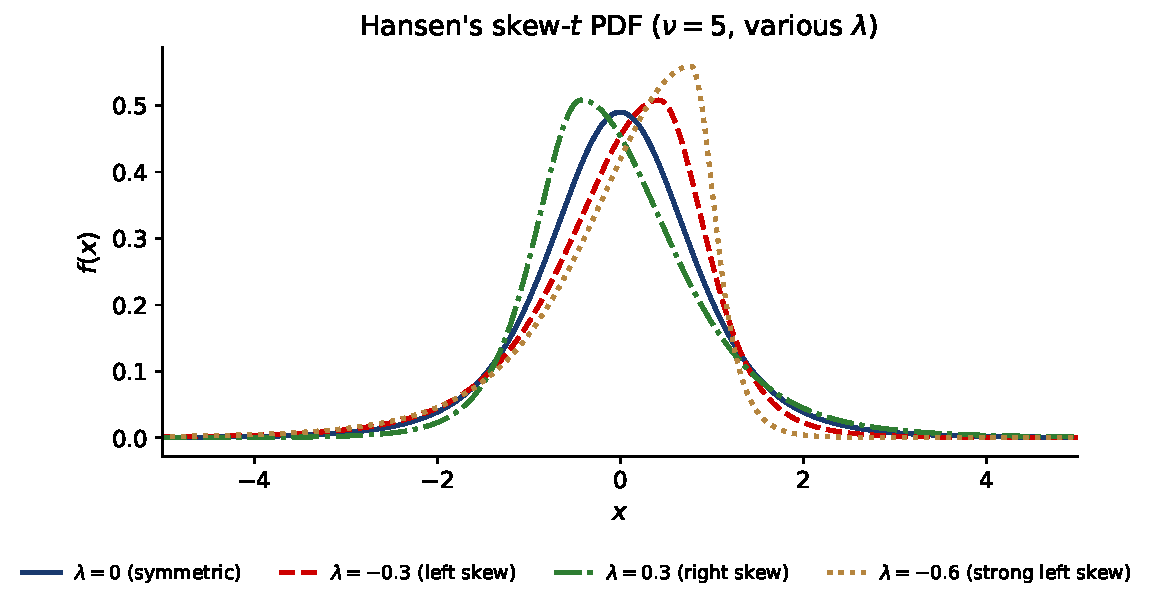
\includegraphics[width=\textwidth]{ch2_skew_t_pdf_theoretical.pdf}
            {\tiny Skew-$t$: asimetrie controlată de $\lambda$}
        \end{column}
    \end{columns}
    \quantlet{SFM\_ch2\_asymmetric\_distributions}{https://github.com/QuantLet/Stat_fin_markets/tree/master/Ch_02/SFM_ch2_asymmetric_distributions}
    \end{cminipage}
\end{frame}

\begin{frame}{Test 2: GED și Laplace}
    \begin{cminipage}{0.95\textwidth}
    \begin{alertblock}{Întrebare}
        GED cu parametrul de formă $\nu = 1$ este echivalentă cu:
    \end{alertblock}
    \begin{block}{Variante de răspuns}
    \begin{itemize}\setlength{\itemsep}{0pt}
        \item \textcolor{MainBlue}{\textbf{(A)}} Distribuția normală
        \item \textcolor{MainBlue}{\textbf{(B)}} Distribuția Laplace
        \item \textcolor{MainBlue}{\textbf{(C)}} Distribuția Cauchy
        \item \textcolor{MainBlue}{\textbf{(D)}} Distribuția uniformă
    \end{itemize}
    \end{block}
    \end{cminipage}
\end{frame}

\begin{frame}{Test 2: Răspuns}
    \begin{cminipage}{0.95\textwidth}
    \begin{columns}[T]
        \begin{column}{0.52\textwidth}
            \begin{exampleblock}{Răspuns: B}
                Distribuția Laplace (double exponential)
            \end{exampleblock}

            \vspace{0.2cm}

            \begin{itemize}\setlength{\itemsep}{0pt}
                \item \textbf{Cazuri speciale GED:}
            \end{itemize}
            \begin{itemize}\setlength{\itemsep}{0pt}
                \item $\nu = 1$: Laplace (cozi grele) \correct
                \item $\nu = 2$: Normal (referință)
                \item $\nu \to \infty$: Uniformă
            \end{itemize}

            \vspace{0.2cm}
            \begin{itemize}\setlength{\itemsep}{0pt}
                \item Verificare:
            \end{itemize}
            \begin{itemize}\setlength{\itemsep}{0pt}
                \item A: $\nu = 2$ \incorrect
                \item C: Cauchy nu este GED \incorrect
                \item D: $\nu \to \infty$ \incorrect
            \end{itemize}
        \end{column}
        \begin{column}{0.45\textwidth}
            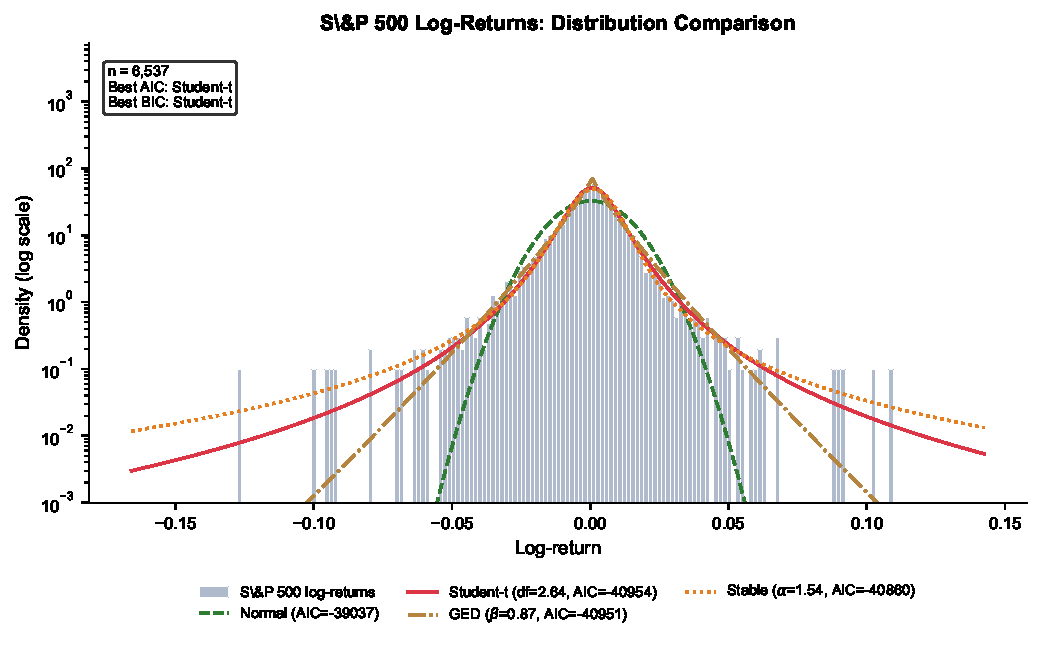
\includegraphics[width=\textwidth]{ch2_dist_comparison_overlay.pdf}
            {\tiny GED: familia parametrică de la Laplace la uniformă}
        \end{column}
    \end{columns}
    \quantlet{SFM\_ch2\_distribution\_comparison}{https://github.com/QuantLet/Stat_fin_markets/tree/master/Ch_02/SFM_ch2_distribution_comparison}
    \end{cminipage}
\end{frame}

\begin{frame}{Test 3: Estimatorul Hill}
    \begin{cminipage}{0.95\textwidth}
    \begin{alertblock}{Întrebare}
        Estimatorul Hill estimează:
    \end{alertblock}
    \begin{block}{Variante de răspuns}
    \begin{itemize}\setlength{\itemsep}{0pt}
        \item \textcolor{MainBlue}{\textbf{(A)}} Media distribuției
        \item \textcolor{MainBlue}{\textbf{(B)}} Varianța distribuției
        \item \textcolor{MainBlue}{\textbf{(C)}} Indicele de coadă $\xi$
        \item \textcolor{MainBlue}{\textbf{(D)}} Parametrul de locație
    \end{itemize}
    \end{block}
    \end{cminipage}
\end{frame}

\begin{frame}{Test 3: Răspuns}
    \begin{cminipage}{0.95\textwidth}
    \begin{columns}[T]
        \begin{column}{0.52\textwidth}
            \begin{exampleblock}{Răspuns: C}
                Indicele de coadă $\xi$ (tail index)
            \end{exampleblock}

            \vspace{0.2cm}

            \begin{itemize}\setlength{\itemsep}{0pt}
                \item \textbf{Formula Hill:}
            \end{itemize}
            $$\hat{\xi}(k) = \frac{1}{k}\sum_{i=1}^{k} \ln\frac{x_{(i)}}{x_{(k+1)}}$$

            \begin{itemize}\setlength{\itemsep}{0pt}
                \item Bazat pe cele mai mari $k$ observații
                \item $\hat{\alpha}_{\text{tail}} = 1/\hat{\xi}$
                \item Hill plot: $\hat{\xi}(k)$ vs $k$
                \item Zona stabilă (platou) $\Rightarrow$ estimare fiabilă
            \end{itemize}
        \end{column}
        \begin{column}{0.45\textwidth}
            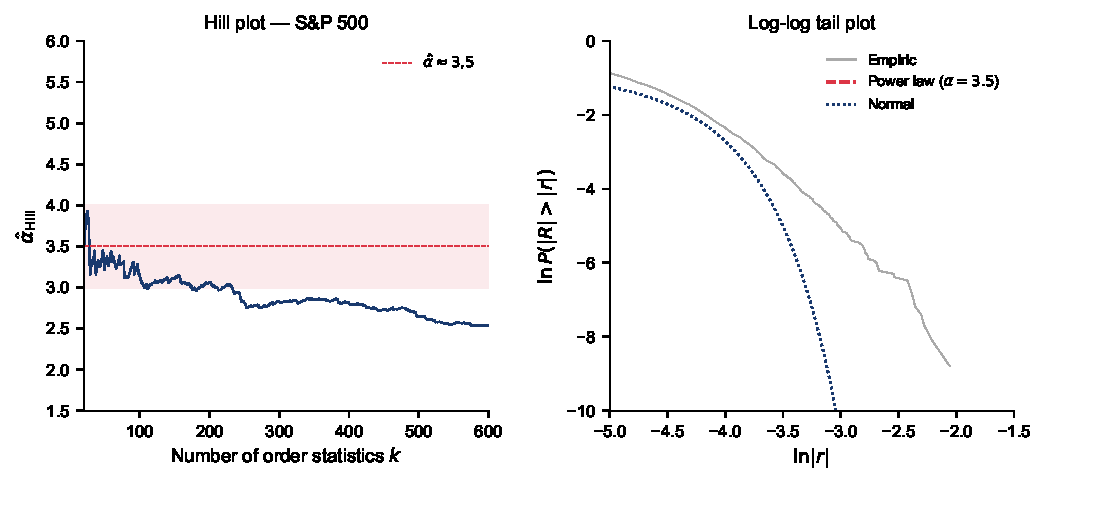
\includegraphics[width=\textwidth]{ch2_hill_plot.pdf}
            {\tiny Hill plot: estimatorul se stabilizează}
        \end{column}
    \end{columns}
    \quantlet{SFM\_ch2\_extreme\_value}{https://github.com/QuantLet/Stat_fin_markets/tree/master/Ch_02/SFM_ch2_extreme_value}
    \end{cminipage}
\end{frame}

\begin{frame}{Test 4: GPD și tipul de coadă}
    \begin{cminipage}{0.95\textwidth}
    \begin{alertblock}{Întrebare}
        În metoda POT, $\xi > 0$ indică:
    \end{alertblock}
    \begin{block}{Variante de răspuns}
    \begin{itemize}\setlength{\itemsep}{0pt}
        \item \textcolor{MainBlue}{\textbf{(A)}} Coadă ușoară (subexponențială)
        \item \textcolor{MainBlue}{\textbf{(B)}} Coadă grea (tip Fr\'{e}chet)
        \item \textcolor{MainBlue}{\textbf{(C)}} Coadă mărginită (tip Weibull)
        \item \textcolor{MainBlue}{\textbf{(D)}} Coadă exponențială (tip Gumbel)
    \end{itemize}
    \end{block}
    \end{cminipage}
\end{frame}

\begin{frame}{Test 4: Răspuns}
    \begin{cminipage}{0.95\textwidth}
    \begin{columns}[T]
        \begin{column}{0.52\textwidth}
            \begin{exampleblock}{Răspuns: B}
                Coadă grea, domeniul de atracție Fr\'{e}chet
            \end{exampleblock}

            \vspace{0.2cm}

            \begin{itemize}\setlength{\itemsep}{0pt}
                \item \textbf{Clasificarea GPD:}
            \end{itemize}
            \begin{itemize}\setlength{\itemsep}{0pt}
                \item $\xi > 0$: Fr\'{e}chet (cozi grele, lege putere) \correct
                \item $\xi = 0$: Gumbel (coadă exponențială)
                \item $\xi < 0$: Weibull (coadă mărginită)
            \end{itemize}

            \vspace{0.2cm}
            \begin{itemize}\setlength{\itemsep}{0pt}
                \item Randamentele financiare: $\xi \in [0.1, 0.4]$, de regulă $\xi \approx 0.2$--$0.3$.
            \end{itemize}
        \end{column}
        \begin{column}{0.45\textwidth}
            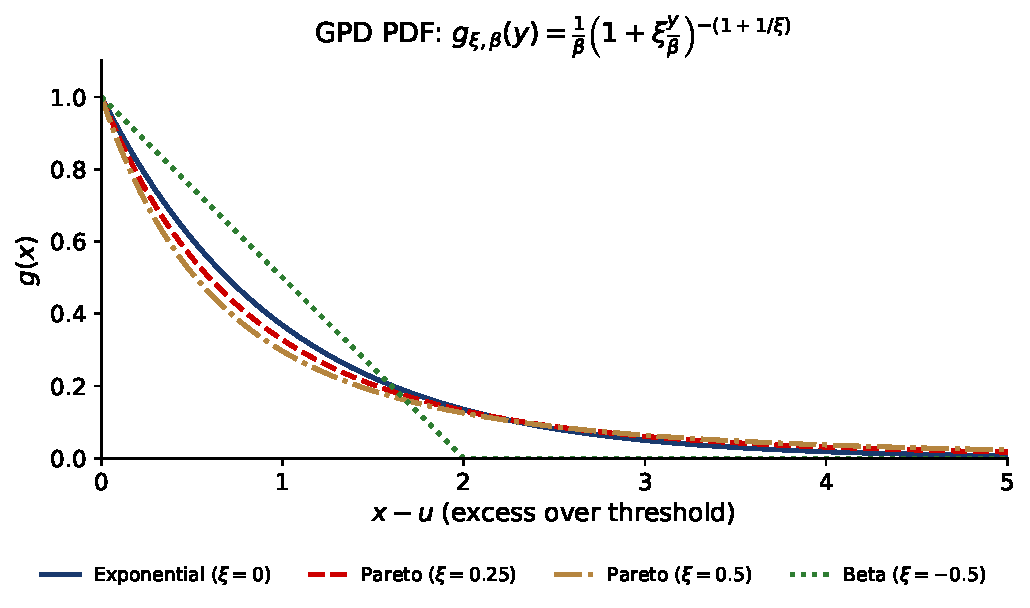
\includegraphics[width=\textwidth]{ch2_gpd_pdf_theoretical.pdf}
            {\tiny GPD: trei tipuri de coadă}
        \end{column}
    \end{columns}
    \quantlet{SFM\_ch2\_extreme\_value}{https://github.com/QuantLet/Stat_fin_markets/tree/master/Ch_02/SFM_ch2_extreme_value}
    \end{cminipage}
\end{frame}

\begin{frame}{Test 5: Graficul Mean Excess}
    \begin{cminipage}{0.95\textwidth}
    \begin{alertblock}{Întrebare}
        Graficul Mean Excess liniar cu pantă pozitivă sugerează:
    \end{alertblock}
    \begin{block}{Variante de răspuns}
    \begin{itemize}\setlength{\itemsep}{0pt}
        \item \textcolor{MainBlue}{\textbf{(A)}} Distribuția normală
        \item \textcolor{MainBlue}{\textbf{(B)}} Distribuția exponențială
        \item \textcolor{MainBlue}{\textbf{(C)}} GPD cu $\xi > 0$ (cozi grele)
        \item \textcolor{MainBlue}{\textbf{(D)}} Absența evenimentelor extreme
    \end{itemize}
    \end{block}
    \end{cminipage}
\end{frame}

\begin{frame}{Test 5: Răspuns}
    \begin{cminipage}{0.95\textwidth}
    \begin{columns}[T]
        \begin{column}{0.52\textwidth}
            \begin{exampleblock}{Răspuns: C}
                GPD cu $\xi > 0$, confirmă cozi grele
            \end{exampleblock}

            \vspace{0.2cm}

            \begin{itemize}\setlength{\itemsep}{0pt}
                \item \textbf{Funcția Mean Excess:}
            \end{itemize}
            $$e(u) = \E[X - u \mid X > u] = \frac{\beta + \xi u}{1 - \xi}$$

            \begin{itemize}\setlength{\itemsep}{0pt}
                \item Interpretare:
            \end{itemize}
            \begin{itemize}\setlength{\itemsep}{0pt}
                \item Pantă pozitivă $\Rightarrow \xi > 0$ (cozi grele) \correct
                \item Pantă zero $\Rightarrow \xi = 0$ (exponențial)
                \item Pantă negativă $\Rightarrow \xi < 0$ (coadă finită)
            \end{itemize}
        \end{column}
        \begin{column}{0.45\textwidth}
            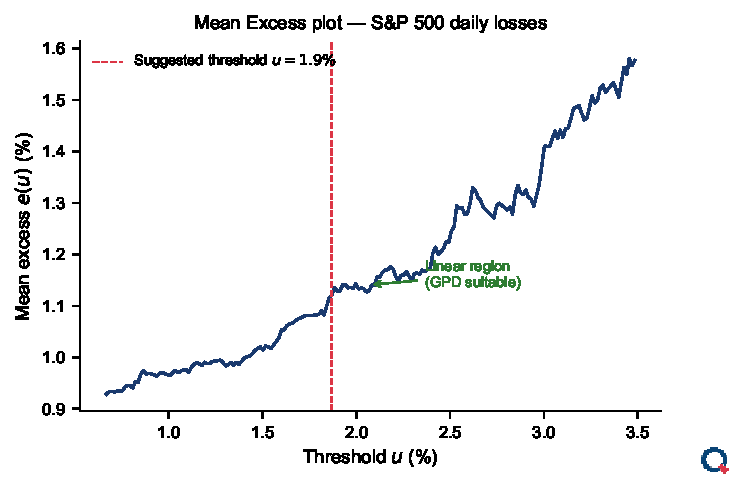
\includegraphics[width=\textwidth]{ch2_mean_excess_plot.pdf}
            {\tiny Mean Excess plot: linearitate $\Rightarrow$ GPD}
        \end{column}
    \end{columns}
    \quantlet{SFM\_ch2\_extreme\_value}{https://github.com/QuantLet/Stat_fin_markets/tree/master/Ch_02/SFM_ch2_extreme_value}
    \end{cminipage}
\end{frame}

\begin{frame}{Test 6: GED --- parametrul de formă}
    \begin{cminipage}{0.95\textwidth}
    \begin{alertblock}{Întrebare}
        GED cu $\nu = 1.3$ comparativ cu distribuția normală ($\nu = 2$) are:
    \end{alertblock}
    \begin{block}{Variante de răspuns}
    \begin{itemize}\setlength{\itemsep}{0pt}
        \item \textcolor{MainBlue}{\textbf{(A)}} Cozi mai ușoare
        \item \textcolor{MainBlue}{\textbf{(B)}} Cozi mai grele
        \item \textcolor{MainBlue}{\textbf{(C)}} Aceleași cozi
        \item \textcolor{MainBlue}{\textbf{(D)}} Nu se poate compara
    \end{itemize}
    \end{block}
    \end{cminipage}
\end{frame}

\begin{frame}{Test 6: Răspuns}
    \begin{cminipage}{0.95\textwidth}
    \begin{columns}[T]
        \begin{column}{0.52\textwidth}
            \begin{exampleblock}{Răspuns: B}
                Cozi mai grele ($\nu < 2 \Rightarrow$ leptokurtosis)
            \end{exampleblock}

            \vspace{0.2cm}

            \begin{itemize}\setlength{\itemsep}{0pt}
                \item \textbf{GED: relația $\nu$ --- cozi:}
            \end{itemize}
            \begin{itemize}\setlength{\itemsep}{0pt}
                \item $\nu < 2$: cozi mai grele decât distribuția normală \correct
                \item $\nu = 2$: normală (referință)
                \item $\nu > 2$: cozi mai ușoare
                \item $\nu = 1$: Laplace (cozi exponențiale)
            \end{itemize}

            \vspace{0.2cm}
            \begin{itemize}\setlength{\itemsep}{0pt}
                \item $P(|X| > 3\sigma)$: Normal $= 0.27\%$, GED($1.3$) $\approx 1.1\%$.
            \end{itemize}
        \end{column}
        \begin{column}{0.45\textwidth}
            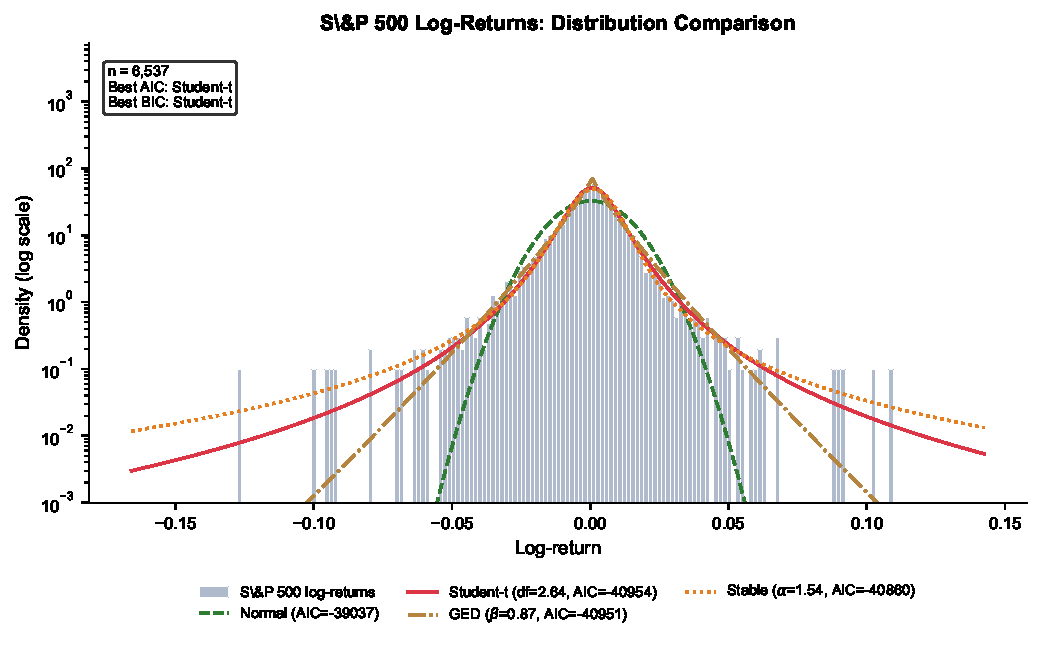
\includegraphics[width=\textwidth]{ch2_dist_comparison_overlay.pdf}
            {\tiny GED: $\nu$ controlează greutatea cozilor}
        \end{column}
    \end{columns}
    \quantlet{SFM\_ch2\_distribution\_comparison}{https://github.com/QuantLet/Stat_fin_markets/tree/master/Ch_02/SFM_ch2_distribution_comparison}
    \end{cminipage}
\end{frame}

\begin{frame}{Test 7: Teorema Fisher--Tippett--Gnedenko}
    \begin{cminipage}{0.95\textwidth}
    \begin{alertblock}{Întrebare}
        Teorema Fisher--Tippett--Gnedenko spune că maximele normate converg la:
    \end{alertblock}
    \begin{block}{Variante de răspuns}
    \begin{itemize}\setlength{\itemsep}{0pt}
        \item \textcolor{MainBlue}{\textbf{(A)}} Distribuția normală
        \item \textcolor{MainBlue}{\textbf{(B)}} Distribuția uniformă
        \item \textcolor{MainBlue}{\textbf{(C)}} Una din trei familii GEV (Fréchet, Gumbel, Weibull)
        \item \textcolor{MainBlue}{\textbf{(D)}} Distribuția Poisson
    \end{itemize}
    \end{block}
    \end{cminipage}
\end{frame}

\begin{frame}{Test 7: Răspuns}
    \begin{cminipage}{0.95\textwidth}
    \begin{columns}[T]
        \begin{column}{0.52\textwidth}
            \begin{exampleblock}{Răspuns: C}
                GEV: trei familii (Fréchet, Gumbel, Weibull)
            \end{exampleblock}

            \vspace{0.2cm}

            \begin{itemize}\setlength{\itemsep}{0pt}
                \item \textbf{Teorema:}
            \end{itemize}
            $$M_n = \max(X_1, \ldots, X_n) \xrightarrow{d} \text{GEV}(\xi)$$

            \begin{itemize}\setlength{\itemsep}{0pt}
                \item $\xi > 0$: Fréchet (cozi grele) \correct
                \item $\xi = 0$: Gumbel (coadă exponențială)
                \item $\xi < 0$: Weibull (coadă mărginită)
            \end{itemize}

            \begin{itemize}\setlength{\itemsep}{0pt}
                \item Analogia cu TLC: TLC $\to$ Normal; FTG $\to$ GEV.
            \end{itemize}
        \end{column}
        \begin{column}{0.45\textwidth}
            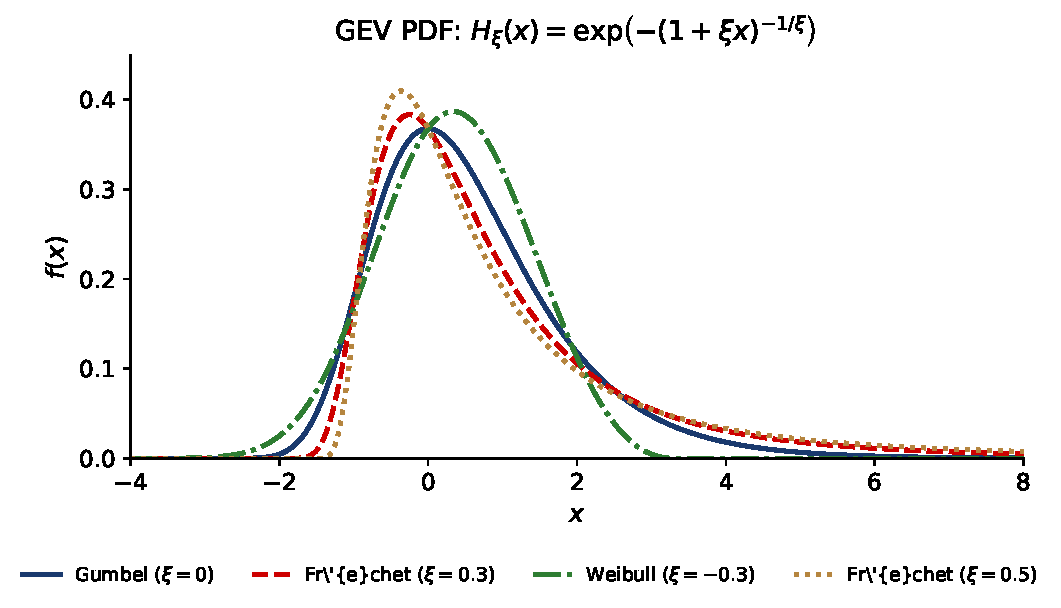
\includegraphics[width=\textwidth]{ch2_gev_pdf_theoretical.pdf}
            {\tiny GEV: cele trei familii de extreme}
        \end{column}
    \end{columns}
    \quantlet{SFM\_ch2\_extreme\_value}{https://github.com/QuantLet/Stat_fin_markets/tree/master/Ch_02/SFM_ch2_extreme_value}
    \end{cminipage}
\end{frame}

\begin{frame}{Test 8: POT vs Block Maxima}
    \begin{cminipage}{0.95\textwidth}
    \begin{alertblock}{Întrebare}
        Avantajul principal al metodei POT față de Block Maxima este:
    \end{alertblock}
    \begin{block}{Variante de răspuns}
    \begin{itemize}\setlength{\itemsep}{0pt}
        \item \textcolor{MainBlue}{\textbf{(A)}} Este mai simplă de implementat
        \item \textcolor{MainBlue}{\textbf{(B)}} Utilizează mai eficient datele extreme
        \item \textcolor{MainBlue}{\textbf{(C)}} Nu necesită alegerea unui prag
        \item \textcolor{MainBlue}{\textbf{(D)}} Funcționează doar pe date normale
    \end{itemize}
    \end{block}
    \end{cminipage}
\end{frame}

\begin{frame}{Test 8: Răspuns}
    \begin{cminipage}{0.95\textwidth}
    \begin{columns}[T]
        \begin{column}{0.52\textwidth}
            \begin{exampleblock}{Răspuns: B}
                POT folosește \textbf{toate} excedentele, nu doar un maxim per bloc
            \end{exampleblock}

            \vspace{0.2cm}

            \begin{itemize}\setlength{\itemsep}{0pt}
                \item \textbf{Comparație:}
            \end{itemize}
            \begin{itemize}\setlength{\itemsep}{0pt}
                \item Block Maxima: un maxim/lună $\Rightarrow$ 12/an
                \item POT: toate excedentele $> u$ $\Rightarrow$ $\sim 50$--$100$/an
            \end{itemize}

            \vspace{0.2cm}
            \begin{itemize}\setlength{\itemsep}{0pt}
                \item Verificare:
            \end{itemize}
            \begin{itemize}\setlength{\itemsep}{0pt}
                \item A: POT este mai complexă \incorrect
                \item C: POT necesită prag $u$ \incorrect
                \item D: POT nu presupune normalitate \incorrect
            \end{itemize}
        \end{column}
        \begin{column}{0.45\textwidth}
            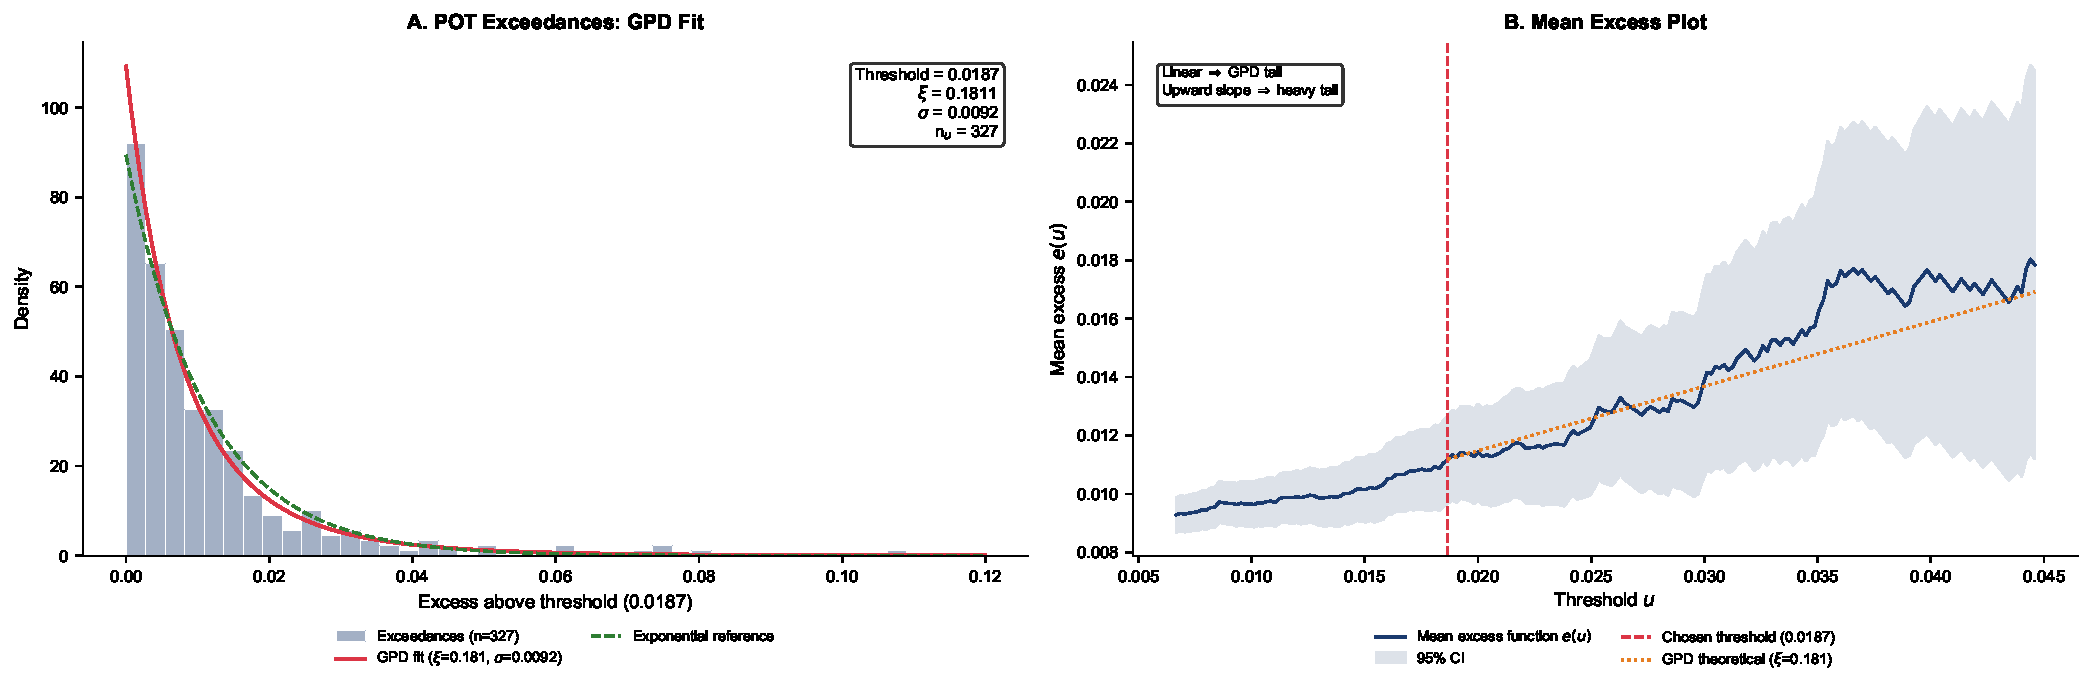
\includegraphics[width=\textwidth]{ch2_evt_gpd_pot.pdf}
            {\tiny POT: mai multe date extreme disponibile}
        \end{column}
    \end{columns}
    \quantlet{SFM\_ch2\_extreme\_value}{https://github.com/QuantLet/Stat_fin_markets/tree/master/Ch_02/SFM_ch2_extreme_value}
    \end{cminipage}
\end{frame}

\begin{frame}{Test 9: Momente și indicele de coadă}
    \begin{cminipage}{0.95\textwidth}
    \begin{alertblock}{Întrebare}
        Dacă $P(X > x) \sim Cx^{-\alpha}$ cu $\alpha = 3$, ce momente există?
    \end{alertblock}
    \begin{block}{Variante de răspuns}
    \begin{itemize}\setlength{\itemsep}{0pt}
        \item \textcolor{MainBlue}{\textbf{(A)}} Doar media
        \item \textcolor{MainBlue}{\textbf{(B)}} Media și varianța, dar nu kurtosis
        \item \textcolor{MainBlue}{\textbf{(C)}} Toate momentele până la ordinul 4
        \item \textcolor{MainBlue}{\textbf{(D)}} Niciun moment nu există
    \end{itemize}
    \end{block}
    \end{cminipage}
\end{frame}

\begin{frame}{Test 9: Răspuns}
    \begin{cminipage}{0.95\textwidth}
    \begin{columns}[T]
        \begin{column}{0.52\textwidth}
            \begin{exampleblock}{Răspuns: B}
                $\E[|X|^p] < \infty$ dacă și numai dacă $p < \alpha$
            \end{exampleblock}

            \vspace{0.2cm}

            \begin{itemize}\setlength{\itemsep}{0pt}
                \item \textbf{Regula momentelor:}
                \item Cu $\alpha = 3$:
            \end{itemize}
            \begin{itemize}\setlength{\itemsep}{0pt}
                \item Media ($p = 1$): $1 < 3$ \correct
                \item Varianța ($p = 2$): $2 < 3$ \correct
                \item Kurtosis ($p = 4$): $4 > 3$ \incorrect
            \end{itemize}

            \vspace{0.2cm}
            \begin{itemize}\setlength{\itemsep}{0pt}
                \item $\Rightarrow$ Sharpe ratio este valid, dar kurtosis-ul eșantionului converge \textbf{foarte lent}.
            \end{itemize}
        \end{column}
        \begin{column}{0.45\textwidth}
            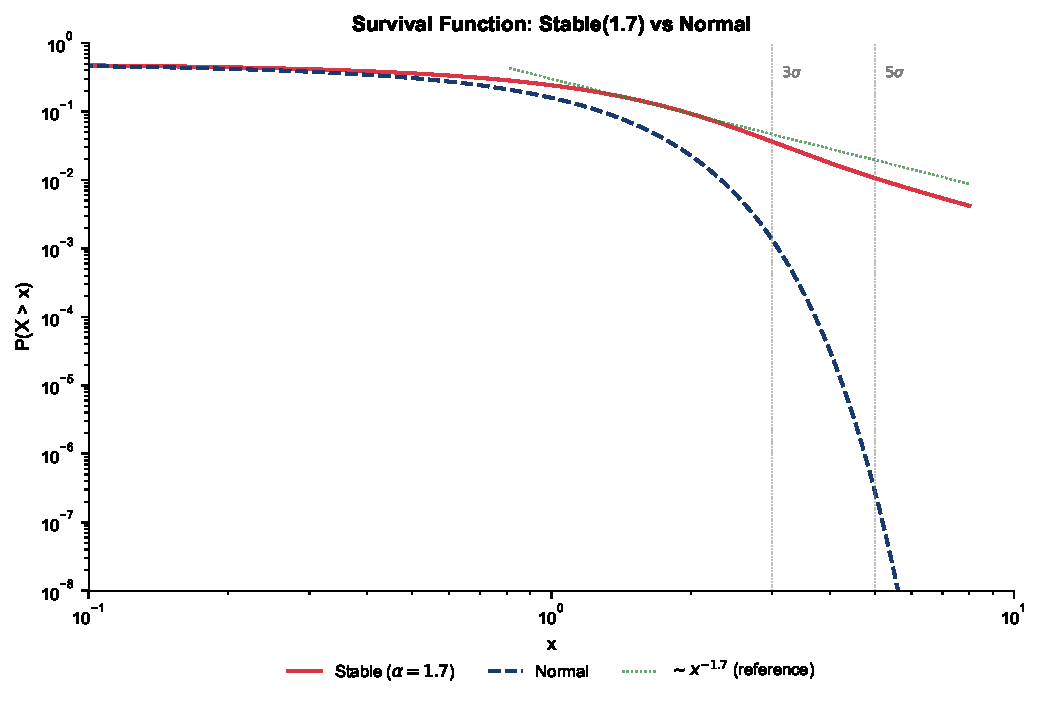
\includegraphics[width=\textwidth]{ch2_tail_survival.pdf}
            {\tiny Legea putere: $P(X>x) \sim x^{-\alpha}$}
        \end{column}
    \end{columns}
    \quantlet{SFM\_ch2\_extreme\_value}{https://github.com/QuantLet/Stat_fin_markets/tree/master/Ch_02/SFM_ch2_extreme_value}
    \end{cminipage}
\end{frame}

\begin{frame}{Test 10: Efectul de levier și Skew-$t$}
    \begin{cminipage}{0.95\textwidth}
    \begin{alertblock}{Întrebare}
        Pe acțiuni, estimarea skew-$t$ dă de regulă $\hat{\lambda} < 0$. Aceasta se datorează:
    \end{alertblock}
    \begin{block}{Variante de răspuns}
    \begin{itemize}\setlength{\itemsep}{0pt}
        \item \textcolor{MainBlue}{\textbf{(A)}} Randamentelor pozitive mai frecvente
        \item \textcolor{MainBlue}{\textbf{(B)}} Efectului de levier (scăderile sunt mai abrupte)
        \item \textcolor{MainBlue}{\textbf{(C)}} Ratei fără risc pozitive
        \item \textcolor{MainBlue}{\textbf{(D)}} Inflației
    \end{itemize}
    \end{block}
    \end{cminipage}
\end{frame}

\begin{frame}{Test 10: Răspuns}
    \begin{cminipage}{0.95\textwidth}
    \begin{columns}[T]
        \begin{column}{0.52\textwidth}
            \begin{exampleblock}{Răspuns: B}
                Efectul de levier (leverage effect)
            \end{exampleblock}

            \vspace{0.2cm}

            \begin{itemize}\setlength{\itemsep}{0pt}
                \item \textbf{Mecanismul (Black, 1976):}
                \item Scăderea prețului $\Rightarrow$ creșterea levierului $\Rightarrow$ creșterea volatilității $\Rightarrow$ scăderi și mai mari.
            \end{itemize}

            \vspace{0.2cm}
            \begin{itemize}\setlength{\itemsep}{0pt}
                \item $\hat{\lambda} < 0$: coada stângă mai grea \correct
                \item Panic selling $>$ FOMO buying
                \item Pe cripto: $\hat{\lambda} \approx 0$ (simetrie)
            \end{itemize}
        \end{column}
        \begin{column}{0.45\textwidth}
            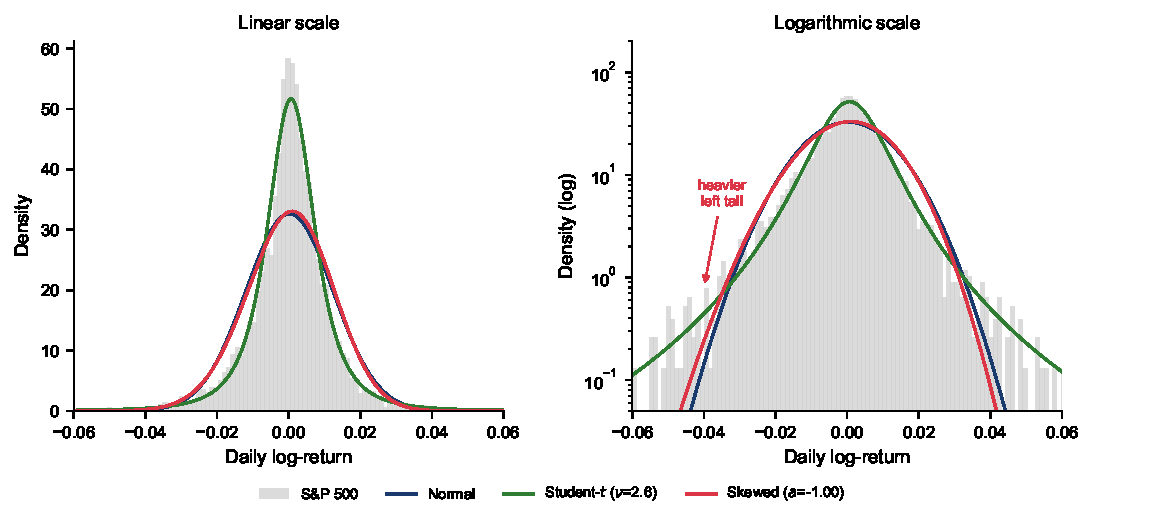
\includegraphics[width=\textwidth]{ch2_skew_t_densities.pdf}
            {\tiny Skew-$t$: asimetrie pe acțiuni}
        \end{column}
    \end{columns}
    \quantlet{SFM\_ch2\_asymmetric\_distributions}{https://github.com/QuantLet/Stat_fin_markets/tree/master/Ch_02/SFM_ch2_asymmetric_distributions}
    \end{cminipage}
\end{frame}

%=============================================================================
% PART 3: TRUE/FALSE QUESTIONS
%=============================================================================
\section{Întrebări Adevărat/Fals}

\begin{frame}{Adevărat sau Fals? --- Întrebări}
    \begin{cminipage}{0.95\textwidth}
    \begin{itemize}\setlength{\itemsep}{0pt}
        \item \textbf{Răspundeți cu Adevărat (A) sau Fals (F):}
    \end{itemize}
    \vspace{0.3cm}
    \begin{enumerate}\setlength{\itemsep}{0pt}
        \item Distribuția skew-$t$ cu $\lambda = 0$ se reduce la Student-$t$ simetrică.
        \item GED cu $\nu < 2$ are cozi mai ușoare decât distribuția normală.
        \item Estimatorul Hill funcționează numai pentru cozi de tip Fr\'{e}chet ($\xi > 0$).
        \item Metoda POT necesită alegerea unui prag $u$, ceea ce o face complet obiectivă.
        \item VaR-POT are justificare teoretică prin teorema Fisher--Tippett--Gnedenko.
        \item EVT-POT poate fi aplicată pe eșantioane foarte mici ($n < 50$).
    \end{enumerate}
    \end{cminipage}
\end{frame}

\begin{frame}{Adevărat sau Fals? --- Răspunsuri}
    \begin{cminipage}{0.95\textwidth}
    \begin{columns}[T]
        \begin{column}{0.55\textwidth}
            \small
            \begin{enumerate}\setlength{\itemsep}{0pt}
                \item \textcolor{Forest}{\textbf{ADEVĂRAT}}: Când $\lambda = 0$, asimetria dispare $\Rightarrow$ simetric
                \vspace{0.1cm}
                \item \textcolor{Crimson}{\textbf{FALS}}: $\nu < 2$ $\Rightarrow$ cozi mai \textit{grele} (leptokurtosis)
                \vspace{0.1cm}
                \item \textcolor{Forest}{\textbf{ADEVĂRAT}}: Hill presupune comportament lege-putere
                \vspace{0.1cm}
                \item \textcolor{Crimson}{\textbf{FALS}}: Alegerea $u$ este \textit{subiectivă}; Mean Excess plot ajută
                \vspace{0.1cm}
                \item \textcolor{Forest}{\textbf{ADEVĂRAT}}: Teorema limită garantează convergența la GPD
                \vspace{0.1cm}
                \item \textcolor{Crimson}{\textbf{FALS}}: EVT necesită suficiente excedente ($N_u \geq 30$--$50$)
            \end{enumerate}
        \end{column}
        \begin{column}{0.42\textwidth}
            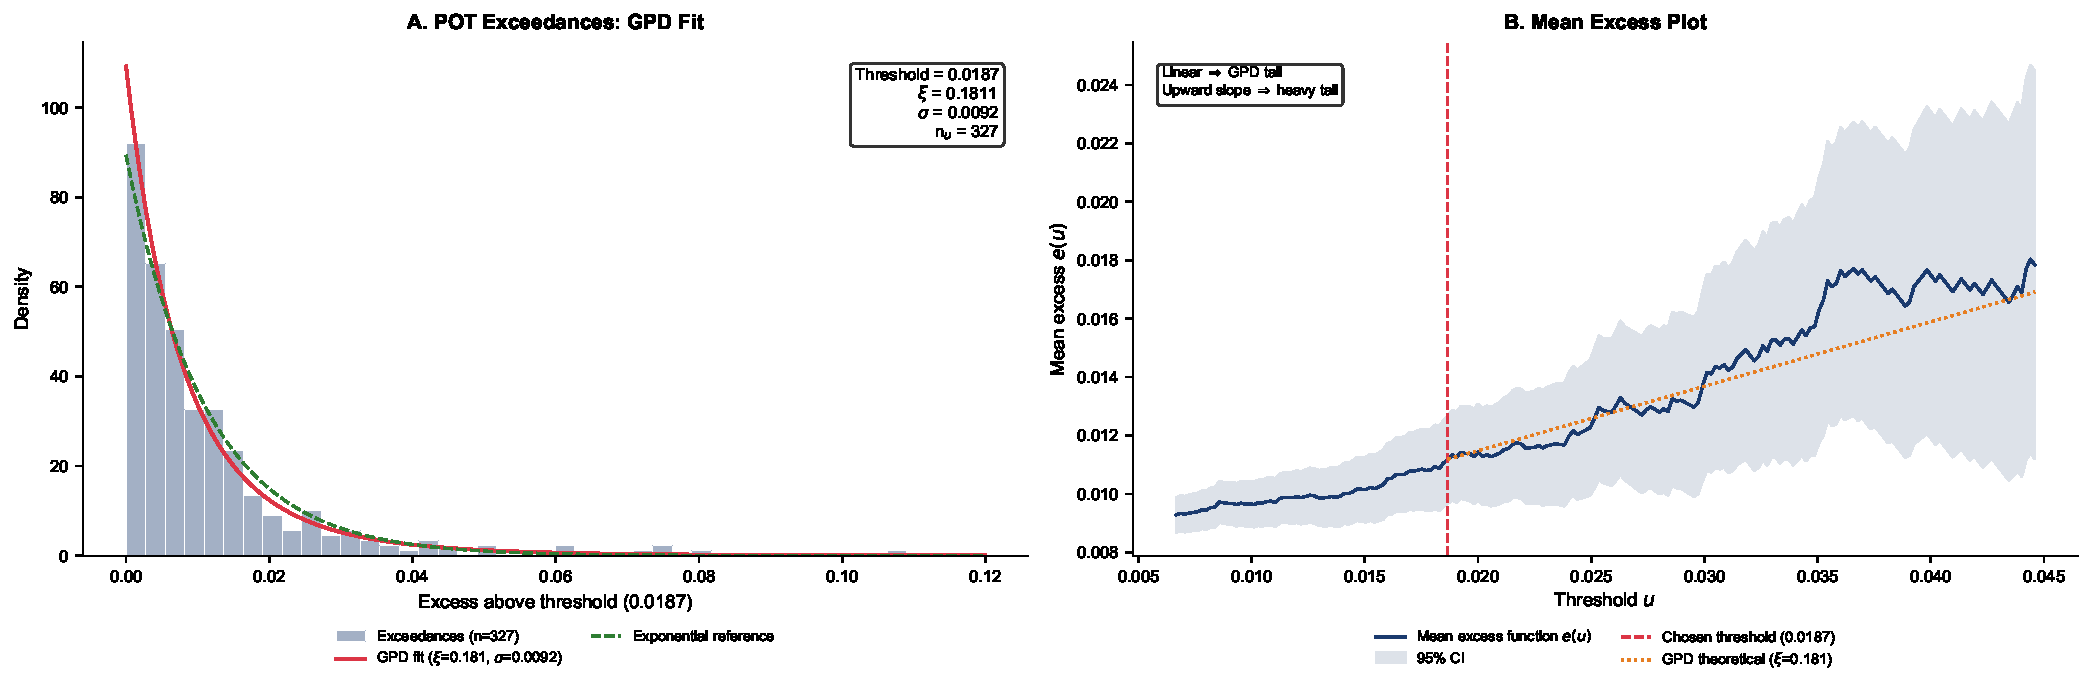
\includegraphics[width=\textwidth]{ch2_evt_gpd_pot.pdf}
            {\tiny EVT-POT: fit GPD pe excedente}
        \end{column}
    \end{columns}
    \quantlet{SFM\_ch2\_extreme\_value}{https://github.com/QuantLet/Stat_fin_markets/tree/master/Ch_02/SFM_ch2_extreme_value}
    \end{cminipage}
\end{frame}

%=============================================================================
% PART 4: CALCULATION EXERCISES
%=============================================================================
\section{Exerciții de Calcul}

\begin{frame}{Exercițiul 1: Skew-$t$ Hansen --- Interpretare}
    \begin{cminipage}{0.95\textwidth}
    \begin{itemize}\setlength{\itemsep}{0pt}
        \item \textbf{Problemă:} Skew-$t$ Hansen cu $\nu = 5$, $\lambda = -0.3$, $\sigma = 1\%$.
        \item Calculați:
    \end{itemize}
    \begin{enumerate}\setlength{\itemsep}{0pt}
        \item VaR la 1\% sub skew-$t$ vs Student-$t$ simetrică
        \item Interpretați diferența în contextul managementului riscului
        \item Ce se întâmplă cu VaR-ul dacă $\lambda$ trece de la $-0.3$ la $+0.3$?
    \end{enumerate}
    \end{cminipage}
\end{frame}

\begin{frame}{Exercițiul 1: Soluție}
    \begin{cminipage}{0.95\textwidth}
    \begin{columns}[T]
        \begin{column}{0.52\textwidth}
            \begin{itemize}\setlength{\itemsep}{0pt}
                \item \textbf{Comparație VaR la 1\% ($\sigma = 1\%$):}
            \end{itemize}

            \renewcommand{\arraystretch}{1.3}
            \begin{tabular}{lc}
            \toprule
            \textbf{Distribuție} & \textbf{VaR 1\%} \\
            \midrule
            Normal & 2.33\% \\
            Student-$t$($\nu = 5$) & 3.36\% \\
            Skew-$t$($\lambda = -0.3$) & 3.89\% \\
            Skew-$t$($\lambda = +0.3$) & 2.91\% \\
            \bottomrule
            \end{tabular}

            \vspace{0.2cm}
            \begin{itemize}\setlength{\itemsep}{0pt}
                \item \textbf{Interpretare:}
            \end{itemize}
            \begin{itemize}\setlength{\itemsep}{0pt}
                \item $\lambda < 0$: VaR crește (coada stângă mai grea)
                \item $\lambda > 0$: VaR scade pe coada stângă
                \item Diferența skew-$t$ vs $t$ simetrică: $\sim 16\%$
            \end{itemize}
        \end{column}
        \begin{column}{0.45\textwidth}
            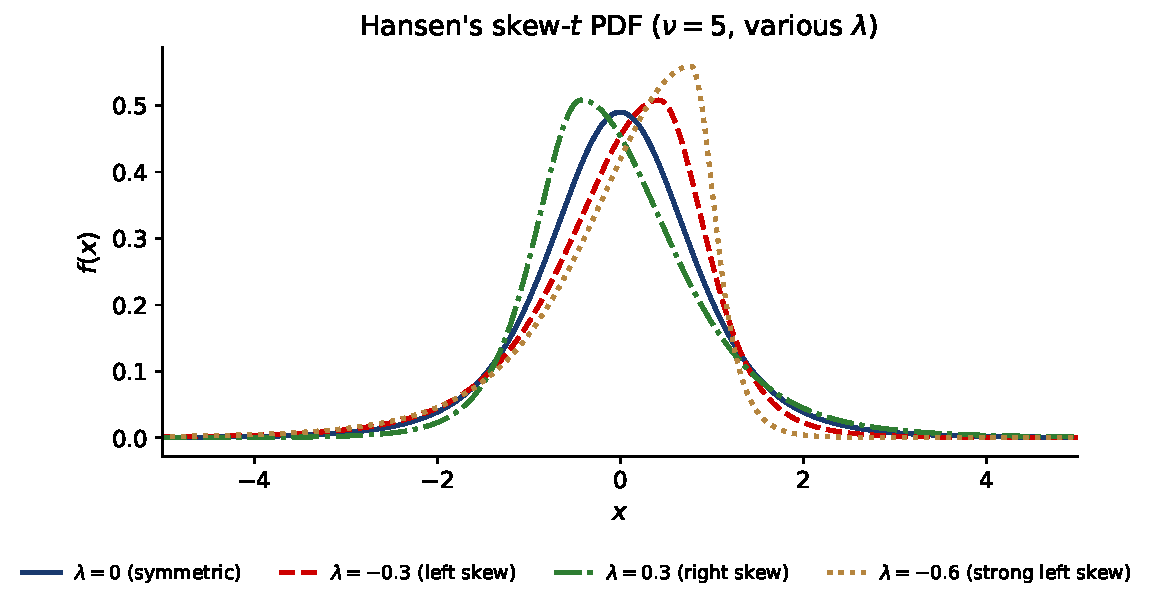
\includegraphics[width=\textwidth]{ch2_skew_t_pdf_theoretical.pdf}
            {\tiny Skew-$t$: coada stângă mai grea ($\lambda < 0$)}
        \end{column}
    \end{columns}
    \quantlet{SFM\_ch2\_asymmetric\_distributions}{https://github.com/QuantLet/Stat_fin_markets/tree/master/Ch_02/SFM_ch2_asymmetric_distributions}
    \end{cminipage}
\end{frame}

\begin{frame}{Exercițiul 2: Estimatorul Hill}
    \begin{cminipage}{0.95\textwidth}
    \begin{itemize}\setlength{\itemsep}{0pt}
        \item \textbf{Problemă:} Din $n = 1000$ observații, cele mai mari 20 valori absolute:
    $x_{(1)} = 5.21$, $x_{(2)} = 4.87$, \ldots, $x_{(20)} = 2.31$, $x_{(21)} = 2.15$.
        \item Calculați:
    \end{itemize}
    \begin{enumerate}\setlength{\itemsep}{0pt}
        \item Estimatorul Hill cu $k = 20$
        \item Indicele de coadă $\hat{\alpha}_{\text{tail}} = 1/\hat{\xi}$
        \item Ce momente există dacă $\hat{\alpha} \approx 2.4$?
    \end{enumerate}
    \end{cminipage}
\end{frame}

\begin{frame}{Exercițiul 2: Soluție}
    \begin{cminipage}{0.95\textwidth}
    \begin{columns}[T]
        \begin{column}{0.52\textwidth}
            \begin{itemize}\setlength{\itemsep}{0pt}
                \item \textbf{1. Estimatorul Hill:}
            \end{itemize}
            $$\hat{\xi}(k) = \frac{1}{k}\sum_{i=1}^{k} \ln\frac{x_{(i)}}{x_{(k+1)}}$$

            \begin{itemize}\setlength{\itemsep}{0pt}
                \item Cu $k = 20$, $x_{(21)} = 2.15$:
                \item Fie $\sum \ln(x_{(i)}/2.15) = 8.42$
            \end{itemize}

            $$\hat{\xi} = 8.42/20 = \textbf{0.421}$$

            \begin{itemize}\setlength{\itemsep}{0pt}
                \item \textbf{2. Indicele:} $\hat{\alpha} = 1/0.421 = \textbf{2.37}$
            \end{itemize}

            \vspace{0.2cm}
            \begin{itemize}\setlength{\itemsep}{0pt}
                \item \textbf{3. Momente:} $\E[|X|^p] < \infty$ dacă $p < \alpha$
            \end{itemize}
            \begin{itemize}\setlength{\itemsep}{0pt}
                \item Media ($p=1$): \textcolor{Forest}{există}
                \item Varianța ($p=2$): \textcolor{Forest}{există}
                \item Kurtosis ($p=4$): \textcolor{Crimson}{nu există}
            \end{itemize}
        \end{column}
        \begin{column}{0.45\textwidth}
            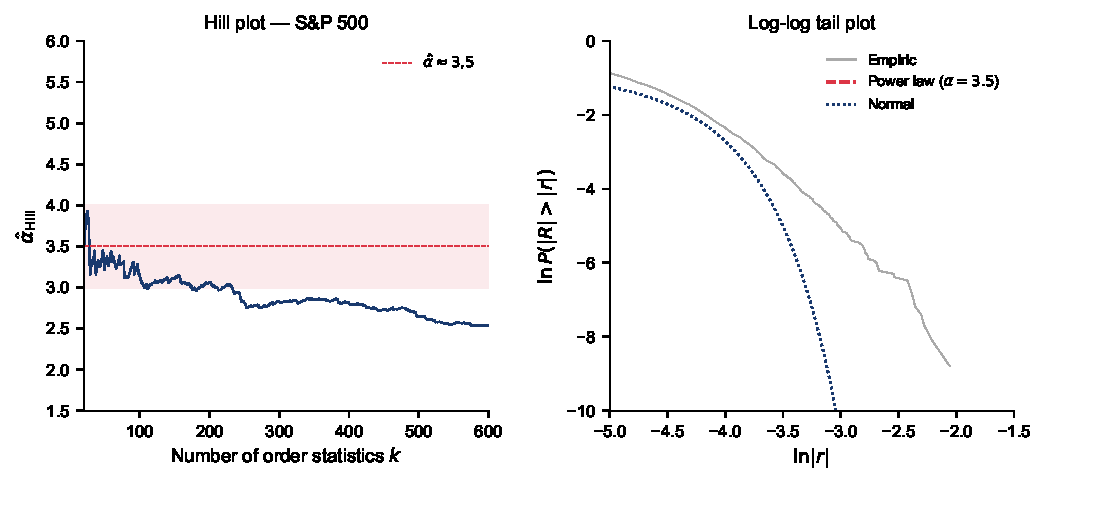
\includegraphics[width=\textwidth]{ch2_hill_plot.pdf}
            {\tiny Hill plot: zona de platou pentru $k$ optim}
        \end{column}
    \end{columns}
    \quantlet{SFM\_ch2\_extreme\_value}{https://github.com/QuantLet/Stat_fin_markets/tree/master/Ch_02/SFM_ch2_extreme_value}
    \end{cminipage}
\end{frame}

\begin{frame}{Exercițiul 3: EVT-POT --- VaR și ES}
    \begin{cminipage}{0.95\textwidth}
    \begin{itemize}\setlength{\itemsep}{0pt}
        \item \textbf{Problemă:} $n = 2000$ pierderi, prag $u$ la percentila 97\% ($u = 2.1\%$), $N_u = 60$, GPD fit: $\hat{\xi} = 0.25$, $\hat{\beta} = 0.8\%$.
        \item Calculați:
    \end{itemize}
    \begin{enumerate}\setlength{\itemsep}{0pt}
        \item VaR-POT la $\alpha = 0.5\%$
        \item ES-POT la $\alpha = 0.5\%$
        \item Comparați cu VaR Normal
    \end{enumerate}
    \end{cminipage}
\end{frame}

\begin{frame}{Exercițiul 3: Soluție}
    \begin{cminipage}{0.95\textwidth}
    \begin{columns}[T]
        \begin{column}{0.52\textwidth}
            \begin{itemize}\setlength{\itemsep}{0pt}
                \item \textbf{1. VaR-POT:}
            \end{itemize}
            $$\text{VaR}_\alpha = u + \frac{\hat{\beta}}{\hat{\xi}}\!\left[\!\left(\frac{n}{N_u}\alpha\right)^{\!-\hat{\xi}} \!\!- 1\right]$$

            \begin{itemize}\setlength{\itemsep}{0pt}
                \item $= 2.1\% + 3.2\%[0.1667^{-0.25} - 1]$
                \item $= 2.1\% + 3.2\% \times 0.565 = \mathbf{3.91\%}$
            \end{itemize}

            \vspace{0.2cm}
            \begin{itemize}\setlength{\itemsep}{0pt}
                \item \textbf{2. ES-POT:}
            \end{itemize}
            $$\text{ES}_\alpha = \frac{\text{VaR}}{1-\hat{\xi}} + \frac{\hat{\beta} - \hat{\xi}u}{1-\hat{\xi}} = \mathbf{5.58\%}$$

            \vspace{0.2cm}
            \begin{itemize}\setlength{\itemsep}{0pt}
                \item \textbf{3.} VaR Normal la 0.5\%: $3.09\%$
                \item Raport: EVT/Normal $= 1.27\times$
            \end{itemize}
        \end{column}
        \begin{column}{0.45\textwidth}
            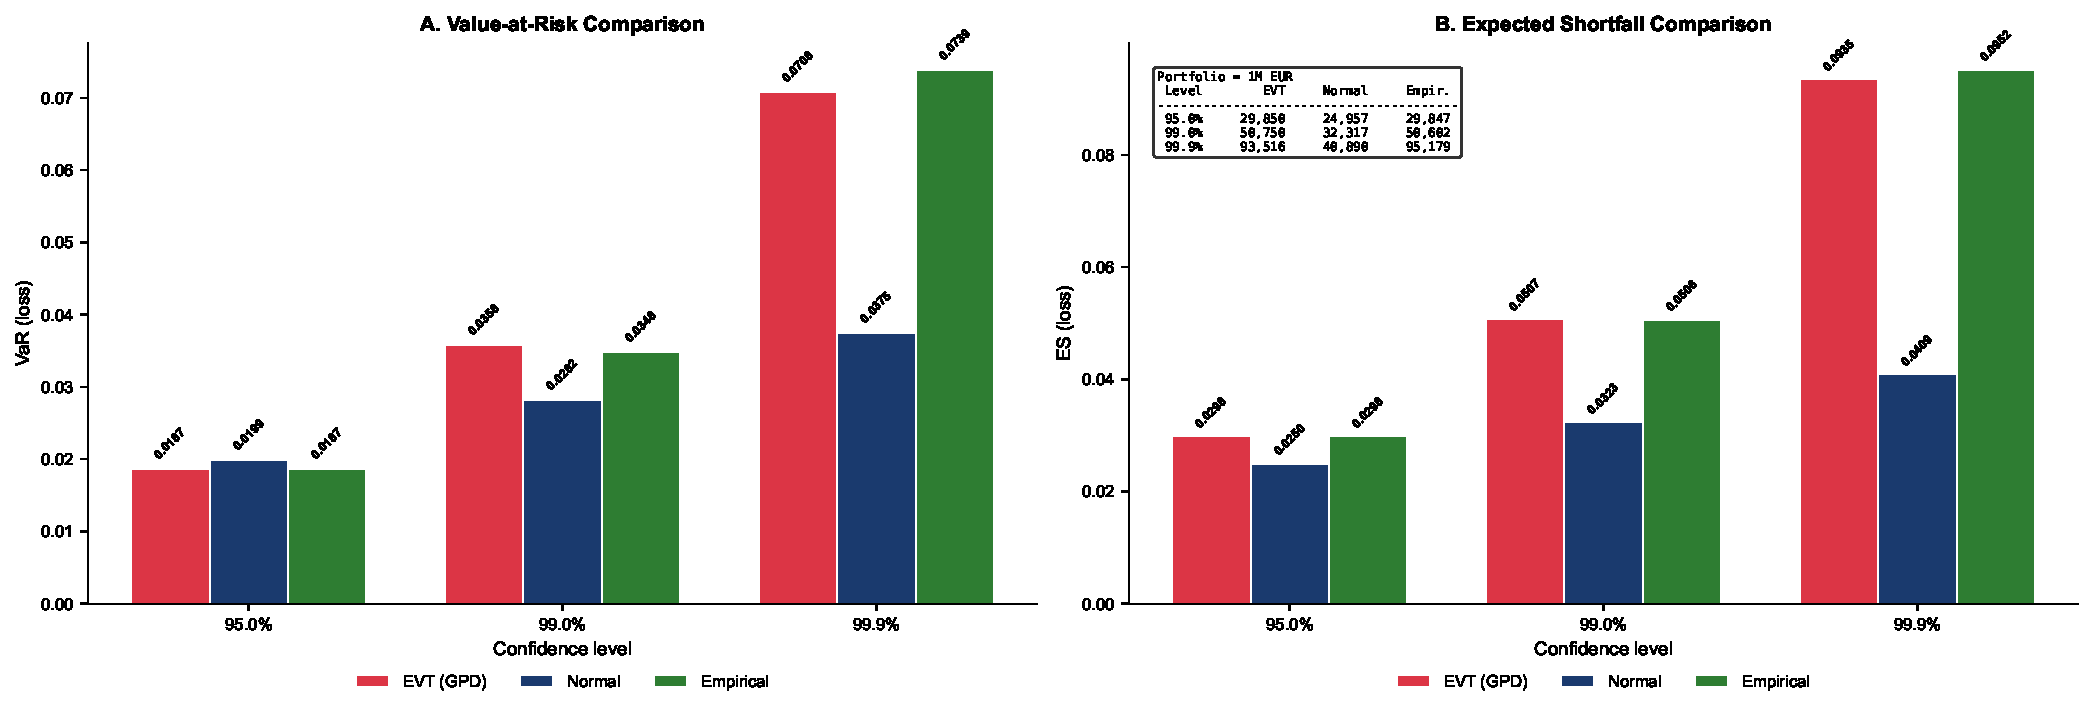
\includegraphics[width=\textwidth]{ch2_evt_var_es.pdf}
            {\tiny EVT: VaR și ES mai conservatoare}
        \end{column}
    \end{columns}
    \quantlet{SFM\_ch2\_extreme\_value}{https://github.com/QuantLet/Stat_fin_markets/tree/master/Ch_02/SFM_ch2_extreme_value}
    \end{cminipage}
\end{frame}

\begin{frame}{Exercițiul 4: GED --- probabilități de coadă}
    \begin{cminipage}{0.95\textwidth}
    \begin{itemize}\setlength{\itemsep}{0pt}
        \item \textbf{Problemă:} GED cu $\hat{\nu} = 1.3$ ajustată pe randamente cu $\sigma = 1\%$.
        \item Calculați:
    \end{itemize}
    \begin{enumerate}\setlength{\itemsep}{0pt}
        \item $P(|X| > 3\sigma)$ sub GED($1.3$) vs Normal
        \item $P(|X| > 5\sigma)$ sub GED($1.3$) vs Normal
        \item Interpretați diferențele pentru managementul riscului
    \end{enumerate}
    \end{cminipage}
\end{frame}

\begin{frame}{Exercițiul 4: Soluție}
    \begin{cminipage}{0.95\textwidth}
    \begin{columns}[T]
        \begin{column}{0.52\textwidth}
            \begin{itemize}\setlength{\itemsep}{0pt}
                \item \textbf{Probabilități de coadă:}
            \end{itemize}

            \renewcommand{\arraystretch}{1.3}
            \begin{tabular}{lcc}
            \toprule
            \textbf{Eveniment} & \textbf{Normal} & \textbf{GED(1.3)} \\
            \midrule
            $|X| > 3\sigma$ & 0.27\% & 1.08\% \\
            $|X| > 5\sigma$ & $5.7 \times 10^{-5}\%$ & 0.042\% \\
            \bottomrule
            \end{tabular}

            \vspace{0.2cm}
            \begin{itemize}\setlength{\itemsep}{0pt}
                \item \textbf{Rapoarte:}
            \end{itemize}
            \begin{itemize}\setlength{\itemsep}{0pt}
                \item La $3\sigma$: GED $= 4\times$ mai probabil
                \item La $5\sigma$: GED $= 737\times$ mai probabil
            \end{itemize}

            \vspace{0.2cm}
            \begin{itemize}\setlength{\itemsep}{0pt}
                \item $\Rightarrow$ GED captează ``Black Swan''-urile pe care distribuția normală le ignoră.
            \end{itemize}
        \end{column}
        \begin{column}{0.45\textwidth}
            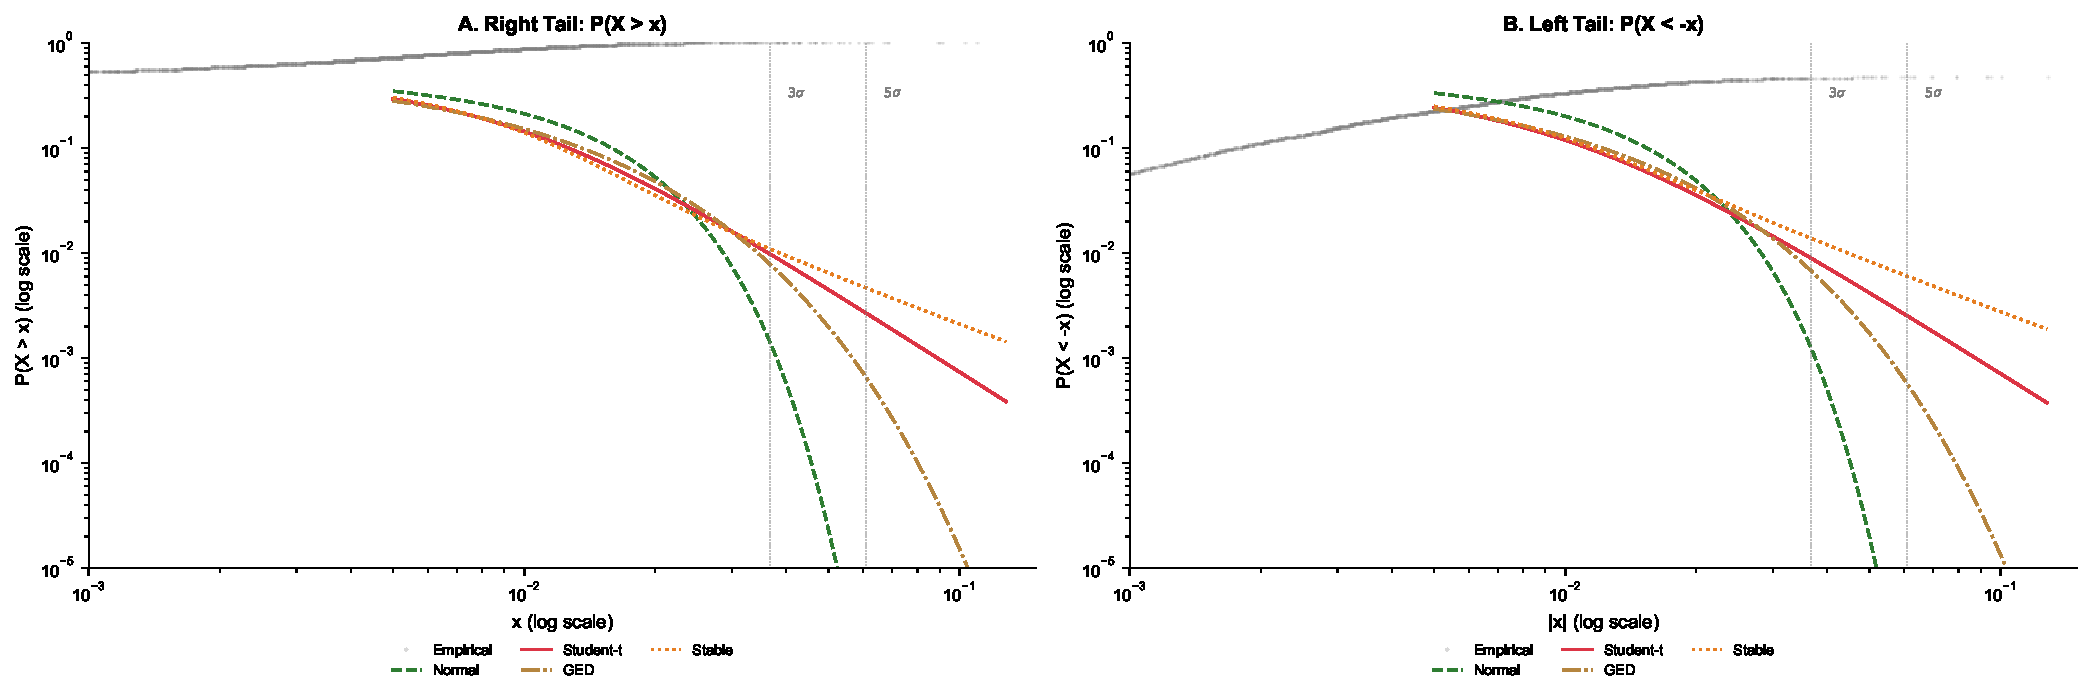
\includegraphics[width=\textwidth]{ch2_dist_comparison_tails.pdf}
            {\tiny Cozile grele: evenimentele extreme sunt mult mai frecvente}
        \end{column}
    \end{columns}
    \quantlet{SFM\_ch2\_distribution\_comparison}{https://github.com/QuantLet/Stat_fin_markets/tree/master/Ch_02/SFM_ch2_distribution_comparison}
    \end{cminipage}
\end{frame}

%=============================================================================
% PART 5: PYTHON EXERCISES
%=============================================================================
\section{Exerciții Python}

\begin{frame}[fragile]{Exercițiu Python 1: Fit GED și Skew-$t$}
    \begin{itemize}\setlength{\itemsep}{0pt}
        \item \textbf{Sarcină:}
    \end{itemize}
    \begin{enumerate}\setlength{\itemsep}{0pt}
        \item Ajustați GED pe randamentele S\&P 500 cu \texttt{scipy.stats.gennorm}
        \item Interpretați parametrul de formă $\hat{\nu}$
        \item Comparați VaR la 1\%: GED vs Normal vs Student-$t$
    \end{enumerate}

    \vspace{0.3cm}
    \begin{itemize}\setlength{\itemsep}{0pt}
        \item \textbf{Cod cheie:}
    \end{itemize}
    \begin{verbatim}
from scipy.stats import gennorm
beta_ged, loc_ged, scale_ged = gennorm.fit(returns)
print(f"GED shape (nu): {beta_ged:.3f}")
var_ged = -gennorm.ppf(0.01, beta_ged, loc_ged, scale_ged)
    \end{verbatim}

    \quantlet{SFM\_ch2\_distribution\_comparison}{https://github.com/QuantLet/Stat_fin_markets/tree/master/Ch_02/SFM_ch2_distribution_comparison}
\end{frame}

\begin{frame}[fragile]{Exercițiu Python 2: Mean Excess Plot și Fit GPD}
    \begin{itemize}\setlength{\itemsep}{0pt}
        \item \textbf{Sarcină:}
    \end{itemize}
    \begin{enumerate}\setlength{\itemsep}{0pt}
        \item Construiți graficul Mean Excess și alegeți pragul $u$
        \item Ajustați GPD pe excedente cu \texttt{scipy.stats.genpareto}
        \item Calculați VaR-POT și ES-POT
    \end{enumerate}

    \vspace{0.3cm}
    \begin{itemize}\setlength{\itemsep}{0pt}
        \item \textbf{Cod cheie:}
    \end{itemize}
    \begin{verbatim}
from scipy.stats import genpareto
losses = -returns[returns < 0].values
u = np.quantile(losses, 0.95)
exceedances = losses[losses > u] - u
xi, _, beta = genpareto.fit(exceedances, floc=0)
var_pot = u + (beta/xi)*((n/n_exceed * alpha)**(-xi) - 1)
    \end{verbatim}

    \quantlet{SFM\_ch2\_extreme\_value}{https://github.com/QuantLet/Stat_fin_markets/tree/master/Ch_02/SFM_ch2_extreme_value}
\end{frame}

\begin{frame}[fragile]{Exercițiu Python 3: Hill Plot}
    \begin{itemize}\setlength{\itemsep}{0pt}
        \item \textbf{Sarcină:}
    \end{itemize}
    \begin{enumerate}\setlength{\itemsep}{0pt}
        \item Construiți Hill plot-ul pe pierderi
        \item Identificați zona de platou și estimați $\hat{\xi}$
        \item Calculați indicele de coadă $\hat{\alpha} = 1/\hat{\xi}$
    \end{enumerate}

    \vspace{0.3cm}
    \begin{itemize}\setlength{\itemsep}{0pt}
        \item \textbf{Funcții cheie:}
    \end{itemize}
    \begin{itemize}\setlength{\itemsep}{0pt}
        \item \texttt{np.sort(losses)[::-1]} pentru sortare descrescătoare
        \item \texttt{np.mean(np.log(top\_k / threshold))} pentru estimator Hill
        \item Zona stabilă: de obicei $k \approx 5\%$--$10\%$ din $n$
    \end{itemize}

    \quantlet{SFM\_ch2\_extreme\_value}{https://github.com/QuantLet/Stat_fin_markets/tree/master/Ch_02/SFM_ch2_extreme_value}
\end{frame}

%=============================================================================
% PART 6: DISCUSSION QUESTIONS
%=============================================================================
\section{Întrebări de Discuție}

\begin{frame}{Discuție 1: Alegerea pragului EVT}
    \begin{cminipage}{0.95\textwidth}
    \begin{itemize}\setlength{\itemsep}{0pt}
        \item \textbf{Scenariu:} Aplicați EVT-POT pe randamentele Bitcoin. Pragul la percentila 90\% dă $\hat{\xi} = 0.35$ ($N_u = 200$), iar la percentila 99\% dă $\hat{\xi} = 0.52$ ($N_u = 20$).
    \end{itemize}

    \vspace{0.3cm}
    \begin{itemize}\setlength{\itemsep}{0pt}
        \item \textbf{Întrebări:}
    \end{itemize}
    \begin{enumerate}\setlength{\itemsep}{0pt}
        \item De ce cele două estimări diferă semnificativ?
        \item Ce prag ați alege și de ce?
        \item Ce rol joacă compromisul bias--varianță?
        \item Cum ați valida alegerea pragului?
    \end{enumerate}
    \end{cminipage}
\end{frame}

\begin{frame}{Discuție 2: Asimetria pierderilor}
    \begin{cminipage}{0.95\textwidth}
    \begin{itemize}\setlength{\itemsep}{0pt}
        \item \textbf{Scenariu:} Pe S\&P 500, estimați: coada stângă $\hat{\xi}_L = 0.28$, coada dreaptă $\hat{\xi}_R = 0.18$. Pe Bitcoin: $\hat{\xi}_L = 0.35$, $\hat{\xi}_R = 0.33$.
    \end{itemize}

    \vspace{0.3cm}
    \begin{itemize}\setlength{\itemsep}{0pt}
        \item \textbf{Întrebări:}
    \end{itemize}
    \begin{enumerate}\setlength{\itemsep}{0pt}
        \item Ce semnifică $\hat{\xi}_L > \hat{\xi}_R$ pe acțiuni?
        \item De ce Bitcoin are cozi aproape simetrice?
        \item Ce implicații are pentru strategiile de hedging?
        \item Cum se leagă această asimetrie de efectul levier?
    \end{enumerate}

    \vspace{0.3cm}
    \begin{itemize}\setlength{\itemsep}{0pt}
        \item \textbf{Indiciu:} Gândiți-vă la mecanismele de piață diferite (panic selling vs FOMO).
    \end{itemize}
    \end{cminipage}
\end{frame}

%=============================================================================
% EXERCIȚIU CU ASISTENȚĂ AI
%=============================================================================
\section{Exercițiu cu asistență AI}

\begin{frame}{Exercițiu AI: Gândire critică}
    \begin{cminipage}{0.95\textwidth}
    \vspace{-3mm}
    \begin{block}{\footnotesize Prompt de testat în ChatGPT / Claude / Copilot}
        {\footnotesize
        ``Descarcă de pe Yahoo Finance datele zilnice S\&P 500 din 2000 până în 2025. Calculează log-randamentele negative (pierderi). Construiește Mean Excess plot. Alege pragul optim. Ajustează GPD pe excedente. Construiește Hill plot. Calculează VaR-POT și ES-POT la 0.5\% și 1\%. Compară cu VaR Normal și Student-t. Vreau cod Python complet cu grafice.''
        }
    \end{block}
    \vspace{-2mm}
    {\footnotesize
    \begin{itemize}\setlength{\itemsep}{0pt}
        \item \textbf{Exercițiu}:
    \end{itemize}
    \begin{enumerate}\setlength{\itemsep}{0pt}
        \item Rulați prompt-ul într-un LLM la alegere și analizați critic răspunsul.
        \item Cum alege pragul $u$? Foloseşte Mean Excess plot sau o regulă arbitrară?
        \item \texttt{genpareto.fit()} este apelat cu \texttt{floc=0}? (Fără, rezultatele sunt greșite.)
        \item Hill plot-ul este construit corect (observații ordonate descrescător)?
        \item ES-POT folosește formula corectă sau o aproximare?
    \end{enumerate}
    }
    \vspace{-2mm}
    \begin{alertblock}{}
        {\footnotesize \textbf{Atenție}: Codul generat de AI poate rula fără erori și arăta profesional. \textit{Asta nu înseamnă că e corect.}}
    \end{alertblock}
    \end{cminipage}
\end{frame}

%=============================================================================
% SUMMARY
%=============================================================================
\section{Rezumat}

\begin{frame}{Concluzii Cheie de Astăzi}
    \begin{cminipage}{0.95\textwidth}
    \begin{enumerate}\setlength{\itemsep}{0pt}
        \item \textbf{Skew-$t$ captează asimetria} --- parametrul $\lambda < 0$ reflectă coada stângă mai grea
        \item \textbf{GED generalizează} --- $\nu < 2$ înseamnă cozi mai grele decât distribuția normală
        \item \textbf{EVT nu presupune o distribuție} globală --- modelează doar coada
        \item \textbf{Hill estimator}: $\hat{\alpha} = [\frac{1}{k}\sum \ln(X_{(i)}/X_{(k+1)})]^{-1}$ estimează indicele de coadă
        \item \textbf{Mean Excess plot liniar} $\Rightarrow$ coadă de tip Pareto (GPD cu $\xi > 0$)
        \item \textbf{VaR-EVT $>$ VaR-Normal} --- cu cât nivelul e mai extrem, cu atât diferența crește
    \end{enumerate}

    \vspace{0.3cm}
    \begin{block}{Următorul Seminar}
        Selecția Modelului și Backtesting VaR
    \end{block}
    \end{cminipage}
\end{frame}

%=============================================================================
% REFERINȚE
%=============================================================================
\begin{frame}{Bibliografie I}
    \begin{cminipage}{0.95\textwidth}
    \begin{block}{Cozi Grele și EVT}
        {\small
        \begin{itemize}\setlength{\itemsep}{0pt}
            \item McNeil, A.J.\ \& Frey, R.\ (2000). ``Estimation of tail-related risk measures,'' \textit{Journal of Empirical Finance}, 7(3-4), 271--300.
            \item Embrechts, P., Klüppelberg, C.\ \& Mikosch, T.\ (1997). \textit{Modelling Extremal Events for Insurance and Finance}. Springer.
            \item Hansen, B.E.\ (1994). ``Autoregressive conditional density estimation,'' \textit{International Economic Review}, 35(3), 705--730.
            \item Hill, B.M.\ (1975). ``A simple general approach to inference about the tail of a distribution,'' \textit{Annals of Statistics}, 3(5), 1163--1174.
        \end{itemize}
        }
    \end{block}
    \end{cminipage}
\end{frame}

\begin{frame}{Surse de Date și Software}
    \begin{cminipage}{0.95\textwidth}
    \begin{block}{Instrumente Software}
        {\small
        \begin{itemize}\setlength{\itemsep}{0pt}
            \item \texttt{scipy.stats} --- GPD fit, distribuții parametrice
            \item \texttt{arch} --- Skew-$t$, GED (pachetul \texttt{arch.univariate.distribution})
            \item \texttt{yfinance} --- Descărcare date financiare
            \item \texttt{matplotlib}, \texttt{seaborn} --- Vizualizare
        \end{itemize}
        }
    \end{block}
    \begin{block}{Date și Exemple}
        {\small
        \begin{itemize}\setlength{\itemsep}{0pt}
            \item S\&P 500, BET, Bitcoin --- descărcate via \texttt{yfinance}
            \item Notebook-uri Jupyter disponibile pe GitHub (QuantLet)
        \end{itemize}
        }
    \end{block}
    \end{cminipage}
\end{frame}

\begin{frame}{Exercițiu de Replicare: McNeil \& Frey (2000)}
    \begin{cminipage}{0.95\textwidth}
        \begin{block}{Obiectiv}
            Replicați analiza EVT-POT din McNeil \& Frey (2000) pe date actuale.
        \end{block}
        \begin{enumerate}\setlength{\itemsep}{2pt}
            {\small
            \item Descărcați randamentele zilnice S\&P 500 (ultimii 20 ani, $\sim$5000 obs.)
            \item Calculați log-pierderile negative și construiți Mean Excess plot
            \item Alegeți pragul $u$ (percentila 95\%) și ajustați GPD pe excedente
            \item Construiți Hill plot-ul și estimați indicele de coadă $\hat{\alpha}$
            \item Calculați VaR-POT și ES-POT la 0.5\% și 1\%
            \item \textbf{Întrebare}: Cum se compară $\hat{\xi}$ pre-2008 vs post-2008?
            }
        \end{enumerate}
        {\tiny Ref: McNeil, A.J.\ \& Frey, R.\ (2000). ``Estimation of tail-related risk measures,'' \textit{Journal of Empirical Finance}, 7(3-4), 271--300.}
    \end{cminipage}
\end{frame}

\begin{frame}{Temă pentru acasă: Seminar 3}
    \begin{cminipage}{0.95\textwidth}
    \begin{block}{Obiectiv}
        Aplicați analiza cozilor grele pe randamentele indicelui BET.
    \end{block}
    \begin{enumerate}\setlength{\itemsep}{2pt}
        {\small
        \item Descărcați randamentele zilnice BET din ultimii 10 ani
        \item Ajustați Skew-$t$ (Hansen) și GED prin MLE, comparați cu Normal/Student-$t$
        \item Construiți Hill plot-ul și estimați indicele de coadă $\hat{\alpha}$
        \item Construiți Mean Excess plot-ul și alegeți pragul $u$
        \item Ajustați GPD pe excedente, calculați VaR-POT și ES-POT la 1\%
        \item Comparați VaR: Normal vs Student-$t$ vs EVT-GPD (tabel)
        \item \textbf{Întrebare}: BET are cozi mai grele sau mai subțiri decât S\&P 500?
        }
    \end{enumerate}
    \quantlet{SFM\_ch2\_case\_study\_2b}{https://github.com/QuantLet/Stat_fin_markets/tree/master/Ch_02/SFM_ch2_case_study_2b}
    \end{cminipage}
\end{frame}

\begin{frame}{}
    \begin{cminipage}{0.95\textwidth}
    \centering
    \Huge\textcolor{IDAred}{Vă mulțumesc!}
    \vspace{1cm}
    \Large\textcolor{MainBlue}{Întrebări?}
    \vspace{0.8cm}
    \normalsize
    Materialele seminarului sunt disponibile la: \url{https://danpele.github.io/SFM/}
    \vspace{0.2cm}
    \href{https://quantlet.com}{\raisebox{-0.15em}{
\includegraphics[height=0.8em]{ql_logo.png}} Quantlet} \hspace{0.5cm}
    \href{https://quantinar.com}{\raisebox{-0.15em}{
\includegraphics[height=0.8em]{qr_logo.png}} Quantinar}
    \end{cminipage}
\end{frame}

\end{document}
